\captionsetup[subfigure]{font={small}, skip=1pt, margin=-0.1cm, singlelinecheck=false}
\section{Results and Discussion} \label{results_cc3} 
\subsection{Computational Cost of RT-CC3 Method} \label{results-cc3-1}
CC3 methods scale at $N^{7}$, making them significantly more expensive compared to CCSD methods. In the implementation, techniques including factorization, reordering, and memory management need to be considered to improve efficiency, while the scaling remains unchanged. Taking the contribution from triples to the $\hat{\Lambda}_{1}$ equation shown in Eq.~(\ref{eq:cc3-y1-exp}) as an example, several adjustments can be made to accelerate the calculation. For contractions involving three tensors, an intermediate consisting of two tensors is calculated first to avoid a $NO^{4}NV^{4}$ contraction. The selection of the two tensors in the initial step may also affect efficiency. For instance, we can rewrite the third term in Eq.~(\ref{eq:cc3-y1-exp}) in two alternatives:
\begin{equation}
\sum\limits_{\substack{jkl\\bcd}}t_{jkl}^{bcd}L_{ij}^{ab}\lambda_{cd}^{kl} = \sum_{klcd}Z_{ikl}^{acd}\lambda_{cd}^{kl},
\end{equation}
where
\begin{equation}
Z_{ikl}^{acd}=\sum_{jb}t_{jkl}^{bcd}L_{ij}^{ab},
\end{equation}
or
\begin{equation}
\sum\limits_{\substack{jkl\\bcd}}t_{jkl}^{bcd}L_{ij}^{ab}\lambda_{cd}^{kl} = \sum_{jb}Z_{j}^{b}L_{ij}^{ab},
\end{equation}
where
\begin{equation}
Z_{j}^{b} = \sum_{klcd}t_{jkl}^{bcd}\lambda_{cd}^{kl}.
\end{equation}
The former approach results in a scaling of $N^{6}$, whereas the intermediate approach requires a contraction that scales at $N^{8}$. The latter approach results in a scaling of $N^{4}$ with an intermediate contraction of $N^{6}$, making it the favorable way to calculate this specific term. For the second term in Eq.~(\ref{eq:cc3-y1-exp}), it can be rewritten as
\begin{equation}
\sum\limits_{\substack{jkl\\bcd}}t_{jkl}^{bcd}\bra{kl}ab \rangle \lambda_{cd}^{ij}=\sum_{jcd}Z_{j}^{acd}\lambda_{cd}^{ij},
\label{eq:cc3-result-l1-term211}
\end{equation}
where
\begin{equation}
Z_{j}^{acd} =\sum_{klb} t_{jkl}^{bcd}\bra{kl}ab \rangle,
\label{eq:cc3-result-l1-term212}
\end{equation}
or
\begin{equation}
\sum\limits_{\substack{jkl\\bcd}}t_{jkl}^{bcd}\bra{kl}ab \rangle \lambda_{cd}^{ij}=\sum_{klb}Z_{ikl}^{b}\bra{kl}ab \rangle,
\end{equation}
where
\begin{equation}
Z_{ikl}^{b} = \sum_{jcd}t_{jkl}^{bcd} \lambda_{cd}^{ij}.
\end{equation}
In this case, the two alternatives share the same scaling of $N^{7}$ for the contraction and $N^{5}$ for the calculation of the intermediates. The former factorization results in a scaling of $NO^{3}NV^{4}$, while the latter one results in a scaling of $NO^{4}NV^{3}$. Following the same approach as was done for the third term in the equation, the latter method should be preferable since $NV$ is usually larger than $NO$ and grows faster when a larger basis set is used. However, it's important to note that the intermediate $Z_{j}^{acd}$ in Eqs.~(\ref{eq:cc3-result-l1-term211}) and~(\ref{eq:cc3-result-l1-term212}) does not contain any $\hat{\Lambda}$ amplitudes. It can be calculated before the iterations and only needs to be computed once during the ground state calculation. Similar considerations are taken into account for the other terms in the CC3 equations as well.

Another computationally expensive step in the RT-CC3 method is the calculation of the occupied-occupied block of the one-electron density, as shown in Eq.~(\ref{eq:cc3-dij}). This calculation involves the contraction of the $\hat{T}_{3}$ and $\hat{\Lambda}_{3}$ amplitudes, which only differ in one index corresponding to the occupied orbital. Nested loops over virtual orbitals are required for this calculation. For the density matrix elements, we choose to implement a two-layer nested loop over virtual orbitals, considering it as a four-index quantity for the triples with two fixed virtual orbitals. This is preferred over a three-index quantity approach with three fixed virtual orbitals. The contraction can be written as
\begin{equation}
\sum_{klc}\Omega_{ilk}^{c}\Omega_{c}^{jlk} \rightarrow D_{ij}
\end{equation}
for a certain pair of virtual orbitals $a,b$. Reducing the number of loops over virtual orbitals accelerates the calculation of the one-electron density substantially. For the ground state calculation, the density needs to be calculated only once after the amplitudes converge from the iterations. Therefore, the effect of this adjustment may not seem to be prominent. However, it is particularly important in RT simulations when the density is calculated in every time step to obtain the corresponding time-dependent properties.

In addition to the above, the permutational symmetry of the amplitudes shown in Eqs.~(\ref{eq:cc3-pijab}) and~(\ref{eq:cc3-pijkabc}), as well as the permutational symmetry of the integrals, are facilitated in both derivation and implementation. Identical terms that only differ in ordering need to be identified to avoid repeated calculation with a polynomial scaling. Regarding the triples, the amplitudes contracted with the same integral or other amplitudes should be reordered first. For instance, in Eq.~(\ref{eq:cc3-x1-exp}), $\hat{T}_{3}$ amplitudes contribute to $\hat{T}_{1}$ amplitudes by contracting with two-electron integrals. Two distinct triples are required in the contraction. Instead of calculating two $\hat{T}_{3}$ amplitudes individually, the amplitudes are reordered so that they share the same set of occupied orbitals. Given the known $t_{ijk}^{abc}$ with a fixed set of $i,j,k$, $t_{ijk}^{cba}$ can be obtained simply by swapping the first and third axis of the 3-index quantity. As noted by Paul et al. in Ref.~\citenum{Paul2020}, the computational time for reordering can be significant depending on the system size and the hardware used for the calculation. Nevertheless, the calculation of an additional triple amplitude is still much more expensive and thereby dominant in computational cost in our implementation. Additionally, it's worth mentioning that the permutational symmetry of the $T_{1}$-transformed integrals no longer has the same symmetry as the regular integrals. The only symmetry rule is that swapping pairs of indices does not change the integral, which is shown as
\begin{equation}
\tilde{\bra{pq}rs \rangle} = \tilde{\bra{qp}sr \rangle}.
\end{equation}
% Table1-CC3-timing
\begin{table} 
    \centering
        \caption{Performance comparison of RT-CC3/cc-pVDZ calculations for water clusters using different hardwares and precisions: double-precision on the CPU (CPU-dp), single-precision on the CPU (CPU-sp), double-precision on the GPU (GPU-dp), and single-precision on the GPU (GPU-sp). Timings (first four columns) are reported in seconds as per-step averages over five time steps. The final three columns indicate speed-ups, calculated as ratios of timings for each case.}
    \begin{tabular}{c|ccccccc}
       \textrm{Water Cluster} & $t_\textrm{CPU-dp}$ &  $t_\textrm{CPU-sp}$ & $t_\textrm{GPU-dp}$ &
$t_\textrm{GPU-sp}$ & $\frac{t_\textrm{CPU-dp}}{t_\textrm{GPU-dp}}$ & $\frac{t_\textrm{CPU-dp}}{t_\textrm{CPU-sp}}$ & 
$\frac{t_\textrm{GPU-dp}}{t_\textrm{GPU-sp}}$ \\ \hline
       \textrm{Monomer} & 14.05 & 15.28 & 19.02 & 18.99 & 0.7387 & 0.9195 & 0.9975 \\ 
       \textrm{Dimer} & 583.4 & 376.5 & 181.6 & 181.7 & 3.213 & 1.550 & 0.9994 \\
       \textrm{Trimer} & 9851 & 5252 & 592.7 & 570.3 & 16.62 & 1.876 & 1.039 \\
       \textrm{Tetramer} & & & 1890 & 1562 & & & 1.210
    \end{tabular}
    \label{tab:cc3-gpu-cpu}
\end{table}

To assess the performance of our RT-CC3 implementation, we calculated the computational time for each time step and presented the results in Table~\ref{tab:cc3-gpu-cpu} for the water monomer, dimer, trimer, and tetramer. Using the cc-pVDZ basis set, a single water molecule has 5 occupied orbitals (NO) and 19 virtual orbitals (NV). Each calculation was conducted exclusively on a single node to ensure consistency in computational resources.

When transitioning from the monomer to the trimer, the system size increases by a factor of 3, theoretically causing the computational time to rise by a factor of $3^7$. As shown in the table, the CPU-dp calculation for the water trimer takes approximately $3^{5.96}$ times longer than the monomer, while the running time of the CPU-sp calculation increases by around $3^{5.32}$. For the GPU calculations, the increase from the monomer to the trimer is approximately $3^{3.130}$ for the double-precision calculation and $3^{3.097}$ for the single-precision case. Furthermore, the GPU-dp calculation for the tetramer takes about $4^{3.317}$ times longer than the monomer, while the single-precision calculation takes approximately $4^{3.181}$ times longer. As the system size continues to grow, the scaling will eventually reach $N^{7}$ as defined.

It is evident that the application of single-precision does not ideally double the calculation speed, especially for GPU implementations. Nevertheless, the speedup from CPU-sp becomes more noticeable as the system size increases, and a discernible speedup emerges for GPU-sp calculations when the system size reaches 96 molecular orbitals. Additionally, a considerable speedup was attained from the GPU implementation overall. For the water trimer, the GPU-dp calculation is 16 times faster than the CPU-dp calculation. We anticipate further speedups from GPUs for even larger systems until a memory limitation is encountered.

\subsection{Optical Properties}\label{results-cc3-2}
\subsubsection{Absorption Spectrum}\label{results-cc3-21}
%Fig1-RTCC3-AbsorptionSpectrum
\begin{figure}
    \centering
    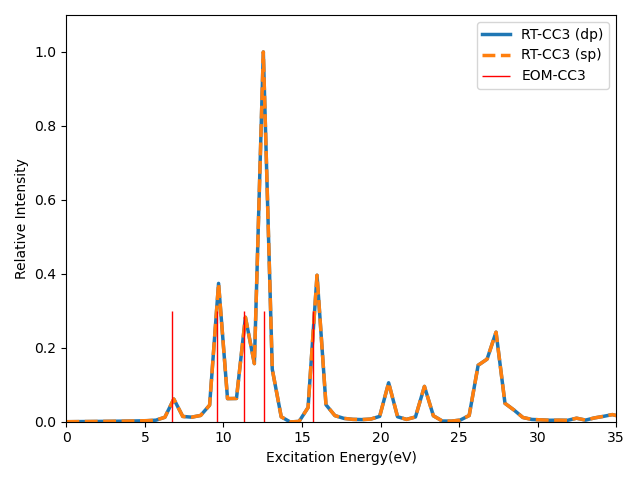
\includegraphics[angle=0, scale=0.43]{ch4/Figs/1-1.png}
    \caption{RT-CC3/cc-pVDZ linear absorption spectrum of \ch{H_{2}O} and corresponding EOM-CC3/cc-pVDZ transitions included as stick-spectra for comparison.}
    \label{fig:abs-water}
\end{figure}
To assess the stability and accuracy of the RT-CC3 implementation, we initially calculated the linear absorption spectrum using the procedure outlined in section~\ref{theory-cc3-21}. To generate a broadband spectrum, a thin Gaussian pulse was applied. The absorption spectrum was computed for both single- and double-precision arithmetics, as depicted in Fig.~\ref{fig:abs-water}. It has been demonstrated that single-precision is sufficient for calculating the absorption spectrum using RT-CCSD in our previous work.\cite{Wang2022} Similarly, in this specific test case, no significant distinction between single- and double-precision results is discernible in the RT-CC3 outcomes. For the EOM-CC3/cc-pVDZ calculation, only excitation energies are attainable from Psi4, while the corresponding oscillator strengths remain unavailable. For illustrative purposes, the `height' of the stick spectra is arbitrarily chosen to enable convenient visualization of the position of each state. However, this choice doesn't convey any information about the probability of the corresponding transition. Through this comparison, we can ascertain that the RT-CC3 method aligns with the EOM-CC3 method.

\subsubsection{Dynamic Polarizabilities and First Hyperpolarizabilities}\label{results-cc3-22}
%Fig2-RTCC3-RCW
\begin{figure}
    \centering
    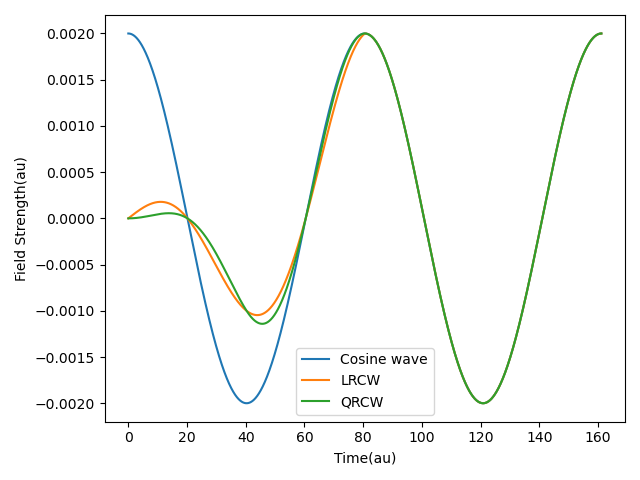
\includegraphics[angle=0, scale=0.43]{ch4/Figs/2-1.png}
    \caption{LRCW and QRCW of two optical cycles. Both of the RCWs have one ramped cycle following a cycle with a regular cosine wave. The frequency and the field strength are 0.078 au and 0.002 au, respectively.}
    \label{fig:rcw}
\end{figure}
As demonstrated in Ref.~\citenum{Ofstad2023}, the QRCW is favorable for extracting optical properties as it has a smoother switch-on compared to the LRCW or a simple oscillatory field without ramping. Fig.~\ref{fig:rcw} illustrates that both LRCW and QRCW have significantly smaller amplitudes at the initial stages of the simulation compared to the regular cosine wave. The QRCW curve exhibits a more gradual increase than the LRCW curve during the first 20 au. Here, we apply both the LRCW and the QRCW to showcase the effect of ramping.

Dynamic polarizabilities and first hyperpolarizabilities of \ch{H_{2}O} at the level of CCSD and CC3 are calculated using finite-difference methods. The simulation with the LRCW spans five ramped cycles, with the first cycle including ramping. In contrast, the simulation with the QRCW encompasses two optical cycles, with ramping applied to the first cycle. The calculations are conducted using both single-precision (sp) and double-precision (dp) arithmetics. A representative result of RT-CCSD/cc-pVDZ (dp) for \ch{H_{2}O} is depicted in Fig.~\ref{fig:pol-hyp-fit} to elucidate the procedure for obtaining polarizabilities and first hyperpolarizabilities. 

From the fitted curve of the time trajectory of the first-order dipole moment, the corresponding polarizability component can be calculated as the amplitude of the curve. As depicted in Fig.~\ref{fig:pol-hyp-fit}, the values of $\alpha_{z}$ at $\omega=0.078$ au are 7.019 au and 7.014 au, respectively, when utilizing the LRCW and QRCW. Regarding the first hyperpolarizabilities, the time trajectory of the second-order dipole moment is fitted into a cosine curve, determining the amplitude $A$ and the phase $B$, which represent the hyperpolarizabilities associated with SHG and OR, respectively. The quality of the curve fitting is assessed using the R$^{2}$ value. As shown in Fig.~\ref{fig:pol-hyp-fit}, a well-fitting curve is characterized by an R$^{2}$ value close to one, whereas a relatively inadequate fitting due to an irregular-shaped second-order dipole trajectory is indicated by an R$^{2}$ value as low as 0.89911. The summarized results are presented in Tables~\ref{tab:polar},~\ref{tab:hyp-shg} and~\ref{tab:hyp-or}.
% Fig3: RT-CC3-pol-hyp-fit
\begin{figure}
     \centering
     \begin{subfigure}{0.47\textwidth}
         \centering
         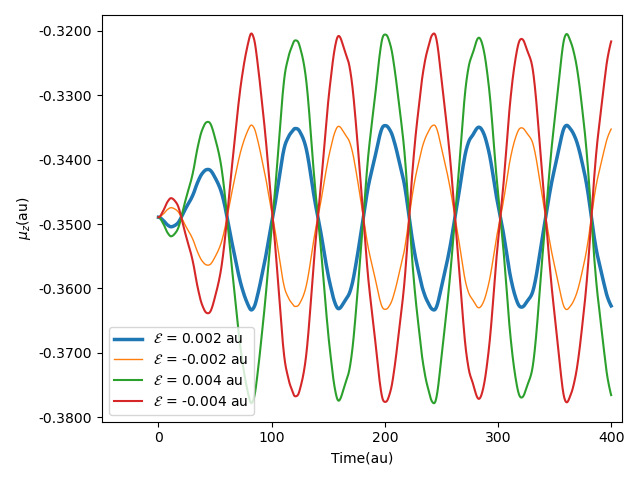
\includegraphics[width=\textwidth]{ch4/Figs/3-1.png}
     \end{subfigure}
     \hfill
     \begin{subfigure}{0.47\textwidth}
         \centering
         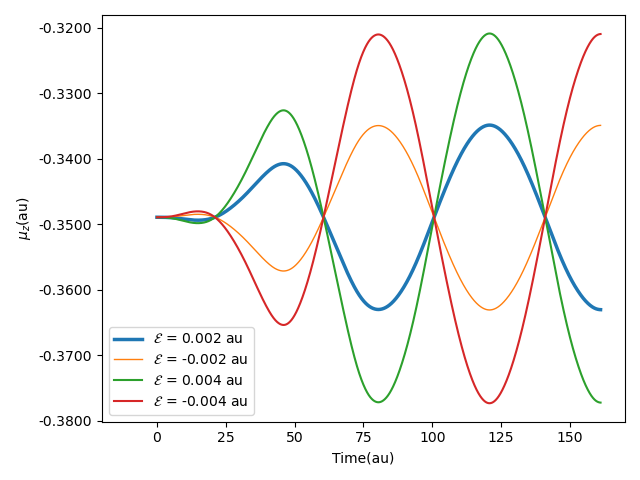
\includegraphics[width=\textwidth]{ch4/Figs/3-4.png}
     \end{subfigure}
     \vfill
     \begin{subfigure}{0.47\textwidth}
         \centering
         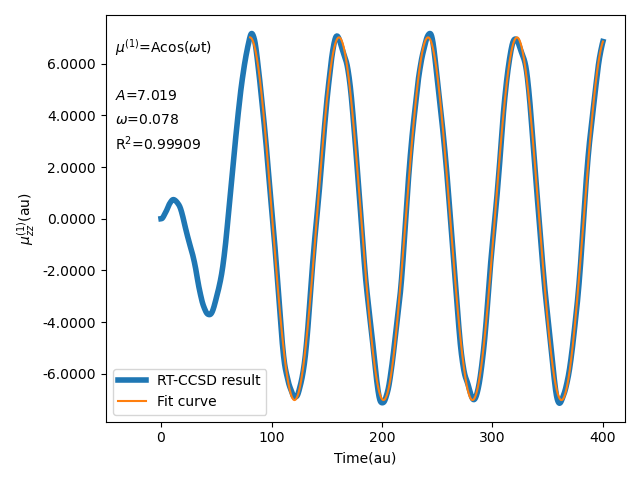
\includegraphics[width=\textwidth]{ch4/Figs/3-2.png}
     \end{subfigure}
     \hfill
     \begin{subfigure}{0.47\textwidth}
         \centering
         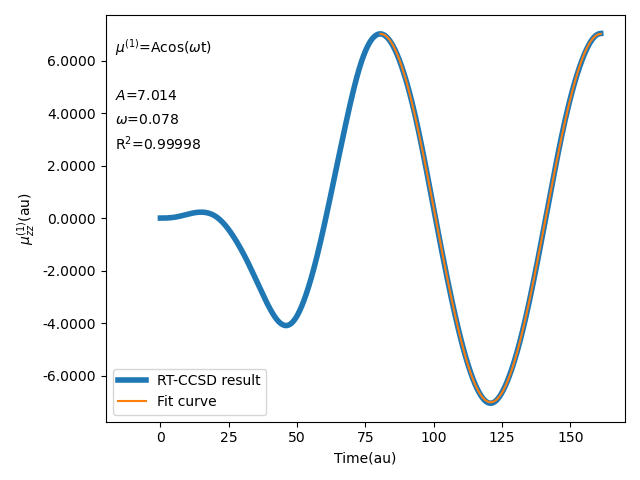
\includegraphics[width=\textwidth]{ch4/Figs/3-5.png}
     \end{subfigure}
     \vfill
     \begin{subfigure}{0.47\textwidth}
         \centering
         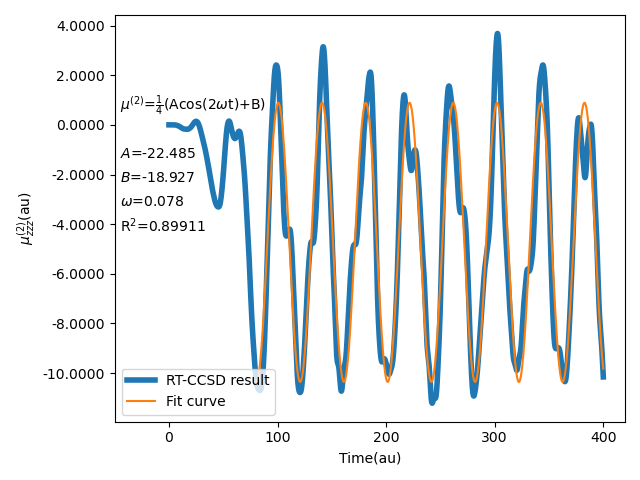
\includegraphics[width=\textwidth]{ch4/Figs/3-3.png}
     \end{subfigure}
     \hfill
     \begin{subfigure}{0.47\textwidth}
         \centering
         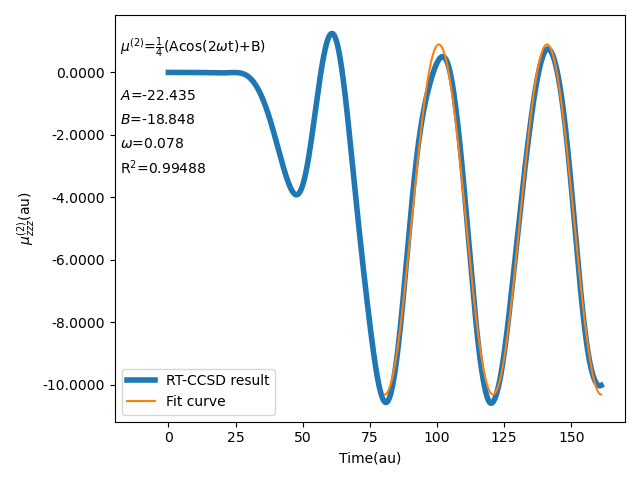
\includegraphics[width=\textwidth]{ch4/Figs/3-6.png}
     \end{subfigure}
     \caption{RT-CCSD/cc-pVDZ (dp) results of \ch{H_{2}O} obtained from four simulations with field strengths of 0.002 au, -0.002 au, 0.004 au, and -0.004 au. The left column displays the LRCW results, including the $z$ component of the induced electric dipole moment, along with the corresponding first- and second-order dipole moments. These are presented from top to bottom along with their fitted curves. The right column showcases the QRCW results.}
     \label{fig:pol-hyp-fit}
\end{figure}

To assess the performance of different simulations, three criteria are evaluated: (1) accuracy compared to linear response (LR) CC, (2) R$^{2}$ value, and (3) simulation length. A method capable of delivering accurate results from a relatively short simulation, along with a curve fitting that yields a high R$^{2}$ value, is the preferable choice. We employ the percentage error to quantify accuracy, which is calculated using the following formula:
\begin{equation}
\textrm{Percentage Error} = |\frac{x - x_{0}}{x_{0}}| \times 100\%,
\end{equation}
where $x$ is the measured value and $x_{0}$ is the reference value. 
% Table2-polarizabilities
\begin{table}
  \centering
  \caption{RT-CCSD/cc-pVDZ and RT-CC3/cc-pVDZ polarizabilities (in atomic units) of \ch{H_{2}O} at 582 nm from simulations with linear ramped continuous wave (LRCW) or quadratic ramped continuous wave (QRCW) fields. Reference values from LR-CCSD and LR-CC3 calculations using CFOUR are provided for comparison. The R$^{2}$ values, indicating the quality of curve fitting, are presented in the last three columns.}
  \begin{tabular}{c|c|ccc|ccc}
                                        & \textrm{Method} & $\alpha_{xx}$ & $\alpha_{yy}$ & $\alpha_{zz}$ 
                                          & R$^{2}_{\alpha_{xx}}$ & R$^{2}_{\alpha_{yy}}$ & R$^{2}_{\alpha_{zz}}$\\
                                          \hline
   & \textrm{LR-CCSD} & 3.182 & 10.549 & 7.017 & & &\\  
    \hline                                     
 \textrm{LRCW}  & \textrm{RT-CCSD\ (dp)} & 3.183 & 10.549 &  7.019 & 0.99980 & 0.99994 & 0.99909 \\
                           & \textrm{RT-CCSD\ (sp)} &  3.183 & 10.549 & 7.019 & 0.99980 & 0.99994 & 0.99909\\
    \cline{1-8}
  \textrm{QRCW} & \textrm{RT-CCSD\ (dp)} & 3.182 & 10.549 &  7.014 & 0.99999 & 0.99994 & 0.99998 \\
                           &\textrm{RT-CCSD\ (sp)} &  3.182 & 10.549 & 7.014 & 0.99999 & 0.99994 & 0.99998\\
    \hline\hline
   & \textrm{LR-CC3} & 3.164 & 10.581 & 7.007 & \\
    \hline
    \textrm{LRCW} &\textrm{RT-CC3\ (dp)} & 3.164 & 10.584 & 7.010 & 0.99981 & 0.99993 & 0.99908 \\
                             &\textrm{RT-CC3\ (sp)} & 3.164 & 10.584 & 7.010 & 0.99981 & 0.99993 & 0.99908 \\
    \cline{1-8}
    \textrm{QRCW} &\textrm{RT-CC3\ (dp)} & 3.165 & 10.580 & 7.004 & 0.99999 & 0.99995 & 0.99998 \\
                             &\textrm{RT-CC3\ (sp)} & 3.165 & 10.580 & 7.004 & 0.99999 & 0.99995 & 0.99998 \\
  \end{tabular}
  \label{tab:polar}
\end{table}

For polarizabilities, the single- and double-precision calculations yield identical results up to three decimal places, with the same R$^{2}$ values accurate for five decimal places. Minor discrepancy can be observed when comparing to the LRCW  and the QRCW results. In RT-CCSD simulations, the LRCW results exhibit a $0.03\%$ error in $\alpha_{xx}$ and a $0.03\%$ error in $\alpha_{zz}$ , while the QRCW results show a $0.04\%$ error in $\alpha_{zz}$. In the case of RT-CC3 simulations, the LRCW results show a $0.03\%$ error in $\alpha_{yy}$ and a $0.05\%$ error in $\alpha_{zz}$ , while the QRCW results indicate a $0.03\%$ error in $\alpha_{xx}$, a $0.01\%$ error in $\alpha_{yy}$ and a $0.05\%$ error in $\alpha_{zz}$. Both of the two ramped continuous waves yield errors well below $0.1\%$. Furthermore, the QRCW requires less simulation time compared to the LRCW and offers a slightly better curve fitting. As a result, the QRCW is the preferred choice, and this conclusion applies to both RT-CCSD and RT-CC3 simulations.
% Table3-hyperpolarizabilities (SHG)
\begin{table}
  \centering
  \caption{RT-CCSD/cc-pVDZ and RT-CC3/cc-pVDZ first hyperpolarizabilities (in atomic units) associated with second harmonic generation (SHG) of \ch{H_{2}O} at 582 nm obtained from simulations with linear ramped continuous wave (LRCW) and quadratic ramped continuous wave (QRCW) fields. Reference values from LR-CCSD calculations using CFOUR are provided. The R$^{2}$ values, reflecting the quality of curve fitting, are displayed in the last three columns.}
  \begin{tabular}{c|c|ccc|ccc}
                                        &  \textrm{Method}  & $\beta_{zxx}$ & $\beta_{zyy}$ & $\beta_{zzz}$ 
                                          & R$^{2}_{\beta_{zxx}}$ & R$^{2}_{\beta_{zyy}}$ & R$^{2}_{\beta_{zzz}}$\\
                                          \hline
    & \textrm{LR-CCSD} & -4.091 & -35.441 & -22.423 & & &\\                 
    \hline                      
     \textrm{LRCW} & \textrm{RT-CCSD\ (dp)} & -4.311 & -35.694 &  -22.485 & 0.93021 & 0.54362 & 0.89911 \\
                              & \textrm{RT-CCSD\ (sp)} & -4.298 & -35.707 & -22.482 & 0.92954 & 0.54195 & 0.89921 \\
    \hline
     \textrm{QRCW} & \textrm{RT-CCSD\ (dp)} & -4.053 & -35.469 &  -22.435 & 0.99892 & 0.97345 & 0.99488 \\
                              & \textrm{RT-CCSD\ (sp)} & -3.987 & -35.520 & -22.447 & 0.99169 & 0.97266 & 0.99480 \\
    \hline\hline
    \textrm{LRCW} & \textrm{RT-CC3\ (dp)} & -3.848 & -36.682 & -21.736 & 0.91595 & 0.67373 & 0.89616 \\
                             & \textrm{RT-CC3\ (sp)} & -3.846 & -36.749 & -22.696 & 0.92203 & 0.67353 & 0.89689 \\
      \hline
     \textrm{QRCW} & \textrm{RT-CC3\ (dp)} & -3.831 & -35.450 & -21.708 & 0.99887 & 0.97111 & 0.99476 \\
                             & \textrm{RT-CC3\ (sp)} & -3.841 & -35.444 & -21.694 & 0.99559 & 0.97180 & 0.99444 \\
  \end{tabular}
  \label{tab:hyp-shg}
\end{table}
% Table4-hyperpolarizabilities (SHG)-error
\begin{table}
  \centering
    \caption{Percentage errors of RT-CCSD/cc-pVDZ first hyperpolarizabilities (au) associated with SHG of \ch{H_{2}O} at 582 nm from calculations using LRCW and QRCW.}
  \begin{tabular}{c|c|ccc}
                                        &  \textrm{Method}  & $\beta_{zxx}$ & $\beta_{zyy}$ & $\beta_{zzz}$ \\
                                          \hline                   
     \textrm{LRCW} & \textrm{RT-CCSD\ (dp)} & 5.38\% & 0.71\% &  0.28\%  \\
                              & \textrm{RT-CCSD\ (sp)} & 5.06\% & 0.75\% & 0.26\%  \\
    \hline
     \textrm{QRCW} & \textrm{RT-CCSD\ (dp)} & 0.93\% & 0.08\% &  0.05\%  \\
                              & \textrm{RT-CCSD\ (sp)} & 2.59\% & 0.22\% & 0.11\%  \\
     \end{tabular}
      \label{tab:hyp-shg-error}
\end{table}
% Table5-hyperpolarizabilities (OR)
\begin{table}
  \centering
    \caption{RT-CCSD/cc-pVDZ and RT-CC3/cc-pVDZ first hyperpolarizabilities (in atomic units) associated with optical rectification (OR) of \ch{H_{2}O} at 582 nm obtained from simulations with linear ramped continuous wave (LRCW) and quadratic ramped continuous wave (QRCW) fields. Reference values from LR-CCSD calculations using CFOUR are provided. The R$^{2}$ values, indicating the quality of curve fitting, are displayed in the last three columns.}
  \begin{tabular}{c|c|ccc|ccc}
                                        &  \textrm{Method}  & $\beta_{zxx}$ & $\beta_{zyy}$ & $\beta_{zzz}$ 
                                          & R$^{2}_{\beta_{zxx}}$ & R$^{2}_{\beta_{zyy}}$ & R$^{2}_{\beta_{zzz}}$\\
                                          \hline
   & \textrm{LR-CCSD} & -4.488 & -30.485 & -18.830 & & &\\  
    \hline                                     
    \textrm{LRCW} & \textrm{RT-CCSD\ (dp)} & -4.532 & -30.568 &  -18.927 & 0.93021 & 0.54362 & 0.89911 \\
                              &   \textrm{RT-CCSD\ (sp)} &  -4.579 & -30.624 & -18.977 & 0.92954 & 0.54195 & 0.89921 \\
    \hline
    \textrm{QRCW} & \textrm{RT-CCSD\ (dp)} & -4.481 & -30.513 &  -18.848 & 0.99892 & 0.97345 & 0.99488 \\
                              &   \textrm{RT-CCSD\ (sp)} &  -4.445 & -30.733 & -18.918 & 0.99169 & 0.97266 & 0.99480 \\
    \hline\hline
     \textrm{LRCW} & \textrm{RT-CC3\ (dp)} & -4.272 & -30.908 & -18.300 & 0.91596 & 0.67373 & 0.89616 \\
                               &   \textrm{RT-CC3\ (sp)} & -4.331 & -30.839 & -18.159 & 0.92203 & 0.67353 & 0.89436 \\
      \hline
      \textrm{QRCW} & \textrm{RT-CC3\ (dp)} & -4.242 & -30.446 & -18.220 & 0.99887 & 0.97111 & 0.99476 \\
                               &   \textrm{RT-CC3\ (sp)} & -4.286 & -30.555 & -18.079 & 0.99559 & 0.97180 & 0.99444 \\
  \end{tabular}
  \label{tab:hyp-or}
\end{table}
% Table6-hyperpolarizabilities (OR)-error
\begin{table}
  \centering
    \caption{Percentage errors of RT-CCSD/cc-pVDZ first hyperpolarizabilities (au) associated with OR of \ch{H_{2}O} at 582 nm from calculations using LRCW and QRCW.}
  \begin{tabular}{c|c|ccc}
                                        &  \textrm{Method}  & $\beta_{zxx}$ & $\beta_{zyy}$ & $\beta_{zzz}$ \\
                                          \hline                   
     \textrm{LRCW} & \textrm{RT-CCSD\ (dp)} & 0.98\% & 0.27\% &  0.51\%  \\
                              & \textrm{RT-CCSD\ (sp)} & 2.03\% & 0.46\% & 0.78\%  \\
    \hline
     \textrm{QRCW} & \textrm{RT-CCSD\ (dp)} & 0.16\% & 0.09\% &  0.10\%  \\
                              & \textrm{RT-CCSD\ (sp)} & 0.96\% & 0.81\% & 0.47\%  \\
     \end{tabular}
  \label{tab:hyp-or-error}
\end{table}

For the first hyperpolarizabilities, we observe larger errors in RT-CCSD results compared to LR-CCSD, as well as differences between single- and double-precision results. This outcome is reasonable, considering that we are calculating a higher-order property involving induced dipole moments. It's important to note that the R$^{2}$ values in Tables~\ref{tab:hyp-shg} and~\ref{tab:hyp-or} are identical. This is because the hyperpolarizabilities associated with second harmonic generation (SHG) and optical rectification (OR) are obtained using the same curve fitting process, with the field applied in a specific direction.

Tables~\ref{tab:hyp-shg-error} and~\ref{tab:hyp-or-error} summarize the percentage errors of hyperpolarizability elements obtained from RT-CCSD calculations, compared to LR-CCSD. In Table~\ref{tab:hyp-shg-error}, the largest error of $5.38\%$ occurs in $\beta_{zxx}$ from the RT-CCSD (dp) calculation using LRCW. By switching to the QRCW, the error in $\beta_{zxx}$ is reduced by $82.71\%$, from $5.8\%$ to $0.93\%$. The percentage errors for other elements are also substantially reduced by at least $48.81\%$. Moreover, the R$^{2}$ values improve when using the QRCW, as seen in Table~\ref{tab:hyp-shg}. Notably, for $\beta_{zyy}$ where the applied field is perpendicular to the molecule's plane, a less smooth trajectory of the second-order dipole moments leads to lower R$^{2}$ values for the LRCW case. Using the QRCW recovers the quality of curve fitting, with R$^{2}$ values exceeding $0.97$.

Regarding precision arithmetic, the double-precision calculation with the LRCW outperforms the single-precision case for $\beta_{zyy}$, while showing slightly worse results for $\beta_{zxx}$ and $\beta_{zzz}$. However, for calculations using the QRCW, the single-precision arithmetic leads to larger errors for all elements. Generally, a double-precision calculation should yield more accurate and robust results because double-precision floating-point numbers are accurate up to 15 decimal places, whereas single-precision numbers are accurate only up to around 7 decimal places. In our test case, when the LRCW is used, the major error arises from the choice of external field. This can be observed from the relatively large overall error and the poor R$^{2}$ values. The difference caused by the two different precision arithmetics is not as pronounced. Neither of them produces sufficiently accurate results. However, when the QRCW is employed, the percentage error is significantly reduced due to the more gradual switch-on of the field, regardless of the chosen precision arithmetics. Consequently, the lower precision arithmetic becomes the primary factor contributing to the resulting error. This is evident in the last two rows of Table~\ref{tab:hyp-shg-error}, where errors in single-precision calculations are 120\% to 178\% larger than those in double-precision calculations.

A similar analysis applies to the results of hyperpolarizabilities associated with OR, as shown in Tables~\ref{tab:hyp-or} and~\ref{tab:hyp-or-error}. In this case, the percentage errors originating from the LRCW are not as significant as those observed in the case of hyperpolarizabilities associated with SHG. Results from the double-precision calculations are consistently more accurate than the single-precision results. Furthermore, the QRCW continues to significantly enhance accuracy for each element, consistent with the trends observed for hyperpolarizabilities associated with SHG.

In the context of RT-CC3 calculations, even though reference values are unavailable for direct comparison, the impact of replacing the LRCW with the QRCW is evident from the substantial increase in R$^{2}$ values. The excellent R$^{2}$ values observed in RT-CC3 calculations involving the QRCW further reinforce the notion that our implementation serves as a viable tool for calculating dynamic polarizability and first hyperpolarizabilities at the CC3 level, given the limitations of available alternatives.

The results presented above demonstrate the capability of the RT-CC3 method for calculating polarizabilities and first hyperpolarizabilities. Given the approximated orbital relaxation with singles in CC3, it is worthwhile to explore a comparison to orbital-optimized coupled cluster (OCC) methods. In time-dependent OCC methods, the singles are replaced by orbital rotations. As an example, Kristiansen et al. implemented real-time (RT) time-dependent orbital-optimized M\o{}ller-Plesset (TDOMP2) theory, which serves as a second-order approximation to the time-dependent orbital-optimized coupled cluster doubles (TDOCCD) method.\cite{Kristiansen2022} TDOMP2 is further compared to RT-CC2, which is a second-order approximation to RT-CCSD. The explicit orbital optimization is proven to be significant for polarizabilities and hyperpolarizabilities, with TDOMP2 outperforming RT-CC2. However, this optimization does not play a critical role in the absorption spectrum, as both methods yield nearly identical spectra.

In addition to the TDOMP2 method, Kristiansen et al. also developed the time-dependent nonorthogonal OCCD (TDNOCCD) method, where the orbital rotation is non-unitary. To assess the performance of RT-CC3 and TDNOCCD for polarizabilities, several ten-electron systems are investigated using double-precision calculations to mitigate errors stemming from low-precision arithmetic. Table~\ref{tab:noccd} presents the TDNOCCD results provided by Kristiansen and compares them with our RT-CC3 results. Reference values include FCI values and LR results, with RT-CCSD results included for comparison. FCI and LR-CC3 values for \ch{Ne} and \ch{HF} are obtained from Ref.~\citenum{Larsen1999}. LR-CC3 values for other molecules are computed using CFOUR. All RT simulations employ the QRCW as the applied field, with one ramped cycle followed by a regular cycle.

For \ch{Ne}, RT-CC3 exhibits good agreement with LR-CC3 and FCI, with errors as large as $0.67\%$ for frequencies ranging from 0.1 au to 0.3 au. However, a notable deviation from LR-CC3/FCI results becomes apparent at a frequency of 0.4 au, which is closer to the resonance at 0.613 au. The accuracy of the result at $\omega=0.5\ au$ is expected to be even lower, as indicated by the comparison between LR-CCSD and RT-CCSD. Surprisingly, the result at $\omega=0.5\ au$ is closer to the reference value. To assess the quality of curve fitting, R$^{2}$ values are compared for different frequencies. The R$^{2}$ values for $\omega=0.3\ au$, $\omega=0.4\ au$, and $\omega=0.5\ au$ are 0.99999, 0.99317, and 0.98147, respectively. These values decrease with higher frequencies. While the result at $\omega=0.5\ au$ is "accurate," it is somewhat less reliable than the results for lower frequencies.

A similar trend is observed for \ch{HF}. RT-CC3 regains accuracy compared to LR-CC3 and FCI at frequencies of 0.1 au and 0.2 au. At a frequency of 0.3 au, which is quite close to the resonance at 0.383 au, the accuracy decreases, resulting in percentage errors of $8.13\%$ and $1.96\%$ for $\alpha_{yy}$ and $\alpha_{zz}$, respectively. Corresponding R$^{2}$ values are 0.97621 and 0.97826, respectively. The error in $\alpha_{zz}$ is slightly smaller than in $\alpha_{yy}$ due to the H-F bond aligning with the z-axis, contributing a nonzero static dipole component, $(\mu_{0})_{z}$. The observed pattern in CC3 results aligns with that in CCSD results.

For \ch{H_{2}O}, selected frequencies are all below the resonance at 0.277 au. RT-CC3 values consistently align with LR-CC3, with only a $0.11\%$ error observed in $\alpha_{zz}$ at $\omega=0.1\ au$. In the case of \ch{NH_{3}}, RT-CC3 results match LR-CC3 values for all frequencies chosen, which are all below the resonance at 0.236 au. The exception is $\alpha_{zz}$ at $\omega=0.1\ au$, where a $0.87\%$ error occurs. This discrepancy contrasts with the agreement between LR-CCSD and RT-CCSD at the same frequency. Notably, the $C_{3}$ axis is aligned with the y-axis, and this significant error is absent in $\alpha_{yy}$.

A similar divergence is seen in the results for \ch{CH_{4}} at the frequency of 0.2 au, whereas the resonance occurs at 0.38 au. RT-CC3 results show a $1.02\%$ deviation from LR-CC3, compared to a mere $0.15\%$ discrepancy in the CCSD case. The corresponding R$^{2}$ values for these two less accurate results, $\alpha_{zz}$ of \ch{NH_{3}} and the polarizability of \ch{CH_{4}}, are 0.99823 and 0.99574, respectively. These values are smaller than those of the other polarizability values, which are all above 0.9999.

To further explore the differences between RT-CCSD and RT-CC3 in these cases, we calculated two additional LR-CCSD/LR-CC3 polarizabilities at different frequencies and performed polynomial regression with five data points. This analysis reveals the relationship between increasing polarizabilities and frequency. In addition to the values listed in Table~\ref{tab:noccd}, $\alpha_{zz}$ of \ch{NH_{3}} is calculated at a frequency of 0.025 au, yielding LR-CC3 and LR-CCSD results of 14.88 au and 14.90 au, respectively. At a frequency of 0.085 au, $\alpha_{zz}$ values are 15.72 au and 15.74 au for LR-CC3 and LR-CCSD, respectively. Two more frequencies, 0.0428 au and 0.15 au, are selected for \ch{CH_{4}}. RT-CC3 and RT-CCSD results at $\omega=0.0428\ au$ are 16.89 au and 16.91 au, respectively. At $\omega=0.15\ au$, the corresponding results are 18.20 au and 18.21 au, respectively.

As shown in Fig.~\ref{fig:polar-polyfit}, polynomial regression closely aligns with data points for all four data sets, with R$^{2}$ values exceeding 0.9999. Moreover, the coefficients of $\omega^{3}$ from LR-CC3 data are larger than those from LR-CCSD data for both \ch{NH_{3}} and \ch{CH_{4}}. The polynomial regression results suggest that CC3 polarizabilities increase slightly faster with frequency compared to CCSD polarizabilities. The impact of frequency moving towards the resonance on polarizability results becomes evident earlier in the frequency range for CC3 compared to CCSD in these test cases, potentially explaining the disagreement observed for polarizability values of \ch{NH_{3}} and \ch{CH_{4}}.

The impact of orbital optimization is explored by comparing TDNOCCD with RT-CCSD and higher levels of theory. As previously mentioned, TDNOCCD differs from RT-CCSD by substituting singles with a non-unitary orbital rotation, where the rotation parameter is time-dependent. OCC-type methods have demonstrated advantages in multi-electron dynamics, chemical bond breaking, response theory, and more.\cite{Pedersen2001, Kohn2005, Sato2018, Pathak2022} Explicit orbital optimization also enhances the stability of real-time simulations when systems are subjected to strong external fields, and the ground state no longer dominates.\cite{Kristiansen2020}

In our test cases, TDNOCCD is initially compared to RT-CCSD by assessing its differences from LR-CCSD. The data presented in Table~\ref{tab:noccd} indicate that TDNOCCD results exhibit relative differences ranging from $0.89\%$ to $7.09\%$, with an average difference of $2.98\%$ across all frequencies and molecules, compared to LR-CCSD. The most significant difference arises from the polarizability of \ch{Ne} at $\omega=0.5\ au$. However, this TDNOCCD result is actually closer to LR-CCSD than RT-CCSD for this specific value. Unlike the RT methods, the frequency dependence of relative differences in TDNOCCD is not as pronounced. It is evident that substantial differences are present not only in high-frequency results but also in low-frequency outcomes, which are distant from resonances. The primary factor contributing to this divergence between TDNOCCD and RT-CCSD, in comparison with LR-CCSD, is the orbital optimization.

Next, TDNOCCD results are compared to LR-CC3 and RT-CC3. Except for a few cases (e.g., \ch{Ne} at $\omega=0.4\ au$ and $0.5\ au$, \ch{HF} at $\omega=0.3\ au$, \ch{NH_{3}} at $\omega=0.1\ au$, and \ch{CH_{4}} at $\omega=0.2\ au$), RT-CC3 results match LR-CC3. However, TDNOCCD deviates from LR-CC3/RT-CC3 by at least $1.03\%$ and up to $3.41\%$, with an average divergence of $2.14\%$. As these polarizability results are unaffected by proximity to resonances, the divergence stems from distinct treatments of orbital optimization and the inclusion/exclusion of triples.

In cases where RT-CC3 exhibits significant percentage errors compared to LR-CC3, the difference between TDNOCCD and LR-CC3 may be larger or smaller than the difference between RT-CC3 and LR-CC3, depending on the RT-CC3 error. When RT-CC3 overestimates polarizability of \ch{Ne} ($\omega=0.4\ au$) and $\alpha_{zz}$ of \ch{HF} ($\omega=0.3\ au$) by $10.54\%$ and $8.13\%$, respectively, TDNOCCD yields smaller values due to orbital optimization, making it closer to LR-CC3. It ultimately underestimates these polarizability values by $2.71\%$ and $0.99\%$, respectively. Orbital optimization's effect mitigates the error and even leads to overcorrection in RT-CC3. However, when RT-CC3 underestimates polarizabilities, the even smaller values from TDNOCCD result in a larger difference from LR-CC3.
% Fig4: polyfit-polar
\begin{figure}
     \centering
     \begin{subfigure}{0.495\textwidth}
         \centering
         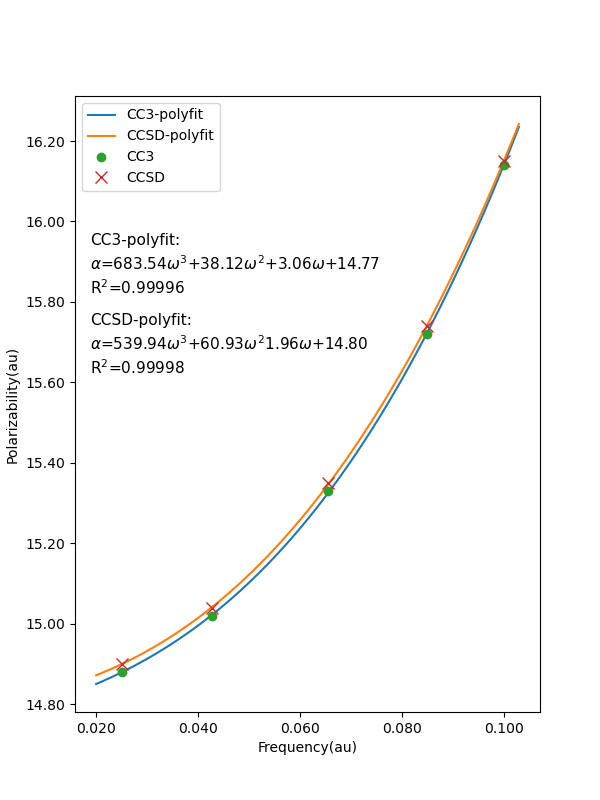
\includegraphics[width=\textwidth]{ch4/Figs/4-1.png}
     \end{subfigure}
     \hfill
     \begin{subfigure}{0.495\textwidth}
         \centering
         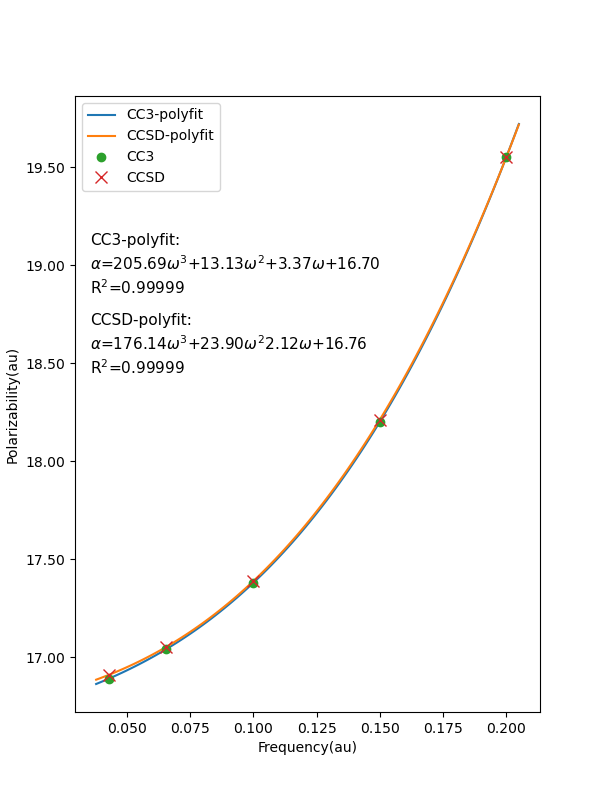
\includegraphics[width=\textwidth]{ch4/Figs/4-2.png}
     \end{subfigure}
     \caption{Variation of $\alpha_{zz}$ values for \ch{NH_{3}} (left) and polarizabilities for \ch{CH_{4}} (right) in relation to frequency, calculated using CC3 and CCSD methods. Polynomial regression curves are depicted, along with the resulting functions and R$^{2}$ values as annotations on the figures.}
     \label{fig:polar-polyfit}
\end{figure}
% Table5-RTCC3-vs-TDNOCCD
\begin{table}
\centering
\caption{Polarizabilities (in atomic units) of \ch{Ne}, \ch{HF}, \ch{H2O}, \ch{NH3} and \ch{CH4}.}
\begin{tabular}{l l r r r r r r r r r}
\hline 
\hline
\ch{Ne}&$\omega\,(\text{a.u.})$ & $0.1$ & $0.2$ & $0.3$ & $0.4$ & $0.5$ \\
\hline
&FCI        &   $2.70$ & $2.79$ & $2.97$ & $3.31$ & $4.09$  \\
&LR-CC3      &   $2.71$ & $2.80$ & $2.98$ & $3.32$ & $4.10$  \\
&RT-CC3      &   $2.71$ & $2.80$ & $2.99$ & $3.67$ & $4.11$  \\
&LR-CCSD     &   $2.74$ & $2.83$ & $3.01$ & $3.38$ & $4.23$  \\		 
&RT-CCSD     &   $2.74$ & $2.83$ & $3.03$ & $3.49$ & $4.76$  \\
&TDNOCCD    &   $2.66$ & $2.75$ & $2.92$ & $3.41$ & $3.93$   \\
\hline
\ch{HF}&$\omega\,(\text{a.u.})$        & \multicolumn{2}{c}{$0.1$}&  \multicolumn{2}{c}{$0.2$} & \multicolumn{2}{c}{$0.3$}            \\ 
&                      & $\alpha_{yy}$   & $\alpha_{zz}$ & $\alpha_{yy}$   & $\alpha_{zz}$ & $\alpha_{yy}$   & $\alpha_{zz}$ \\
\hline
&FCI      & $4.39$ & $6.33$ & $4.76$ & $6.74$ & $6.00$ & $7.63$ \\
&LR-CC3    & $4.39$ & $6.34$ & $4.77$ & $6.76$ & $6.03$ & $7.64$ \\ 
&RT-CC3    & $4.39$ & $6.34$ & $4.77$ & $6.76$ & $6.52$ & $7.49$ \\ 
&LR-CCSD   &     $4.44$      &   $6.41$  &     $4.83$      &  $6.83$ &     $6.19$      &   $7.73$          \\
&RT-CCSD   & $4.45$ & $6.41$ & $4.84$ & $6.83$ & $6.72$ & $7.84$\\
&TDNOCCD  & $4.30$ & $6.21$ & $4.63$ & $6.60$ & $6.09$ & $7.35$ \\
\hline
\ch{H2O} & $\omega\,(\text{a.u.})$ & \multicolumn{3}{c}{$0.0428$} & \multicolumn{3}{c}{$0.0656$} & \multicolumn{3}{c}{$0.1$} \\
&                      & $\alpha_{xx}$          & $\alpha_{yy}$   & $\alpha_{zz}$ & $\alpha_{xx}$  & $\alpha_{yy}$   & $\alpha_{zz}$ & $\alpha_{xx}$  & $\alpha_{yy}$   & $\alpha_{zz}$ \\
\hline 
&LR-CC3   &     $8.72$    &     $9.86$       &   $9.04$      &     $8.83$    &     $9.92$       &   $9.12$      &     $9.10$    &     $10.06$      &   $9.30$\\
&RT-CC3   &     $8.72$    &     $9.86$       &   $9.04$      &     $8.83$    &     $9.92$      &   $9.12$      &     $9.10$    &     $10.06$      &   $9.31$\\
&LR-CCSD   &     $8.78$    &     $9.93$       &   $9.11$      &     $8.89$    &     $9.99$       &   $9.19$      &     $9.18$    &     $10.14$      &   $9.37$\\
&RT-CCSD   &     $8.78$    &     $9.93$       &   $9.11$      &     $8.90$    &     $10.00$      &   $9.19$      &     $9.19$    &     $10.14$      &   $9.37$\\
&TDNOCCD  &     $8.45$       &   $9.67$               & $8.84$              &  $8.55$             &  $9.73$                &   $8.90$            &     $8.79$    &     $9.86$       &   $9.07$\\
\hline
\ch{NH3} & $\omega\,(\text{a.u.})$        & \multicolumn{2}{c}{$0.0428$} & \multicolumn{2}{c}{$0.0656$} & \multicolumn{2}{c}{$0.1$} \\
&        & $\alpha_{yy}$   & $\alpha_{zz}$ & $\alpha_{yy}$& $\alpha_{zz}$ & $\alpha_{yy}$& $\alpha_{zz}$ \\
\hline 
&LR-CC3   &      $13.05$    &    $15.02$    & $13.15$      &   $15.33$     & $13.39$      & $16.14$       \\
&RT-CC3   &      $13.05$    &    $15.02$    & $13.15$      &   $15.33$     & $13.38$      & $16.00$       \\
&LR-CCSD   &      $13.10$    &    $15.04$    & $13.20$      &   $15.35$     & $13.44$      & $16.15$       \\
&RT-CCSD   &      $13.10$    &    $15.05$    & $13.20$      &   $15.36$     & $13.45$      & $16.15$       \\
&TDNOCCD  &      $12.85$    &    $14.57$    & $12.94$      &   $14.84$     & $13.17$      & $15.51$       \\
\hline
\ch{CH4}&$\omega\,(\text{a.u.})$ & $0.0656$ & $0.1$ & $0.2$\\
\hline
&LR-CC3   & $17.04$ & $17.38$ & $19.55$ \\ 
&RT-CC3   & $17.04$ & $17.37$ & $19.35$ \\
&LR-CCSD   & $17.05$ & $17.39$ & $19.55$ \\ 
&RT-CCSD   & $17.05$ & $17.39$ & $19.58$ \\
&TDNOCCD  & $16.86$ & $17.19$ & $19.22$ \\
\hline 
\hline
\end{tabular}
\label{tab:noccd}
\end{table}

% G' tensor 
\subsubsection{$G'$ tensor}\label{results-cc3-23}
% Fig5: RT-CC3-G' tensor
\begin{figure}
     \centering
     \begin{subfigure}{0.47\textwidth}
         \centering
         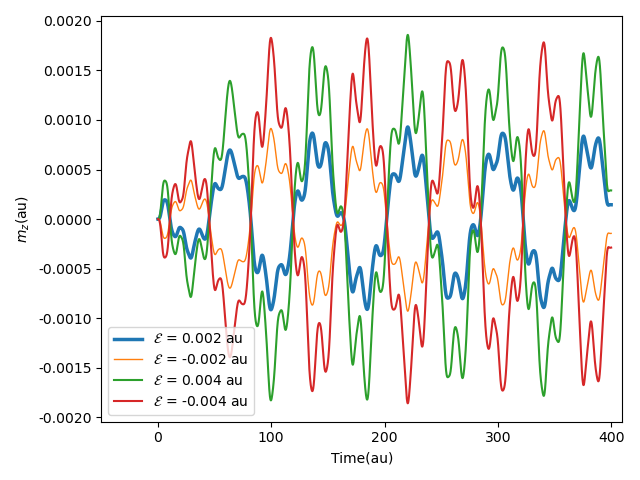
\includegraphics[width=\textwidth]{ch4/Figs/5-1.png}
     \end{subfigure}
     \hfill
     \begin{subfigure}{0.47\textwidth}
         \centering
         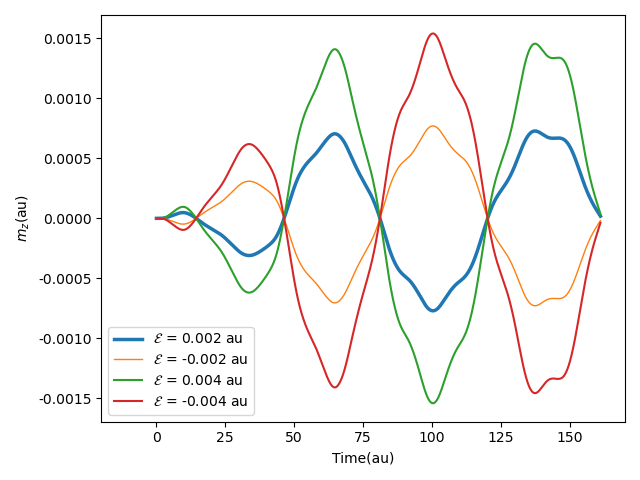
\includegraphics[width=\textwidth]{ch4/Figs/5-3.png}
     \end{subfigure}
     \vfill
     \begin{subfigure}{0.47\textwidth}
         \centering
         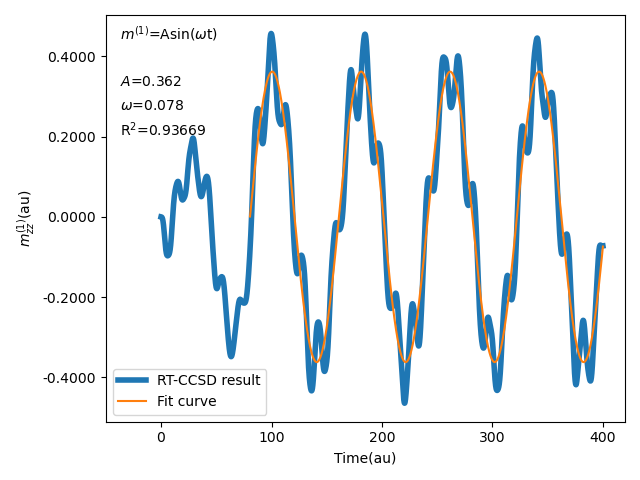
\includegraphics[width=\textwidth]{ch4/Figs/5-2.png}
     \end{subfigure}
     \hfill
     \begin{subfigure}{0.47\textwidth}
         \centering
         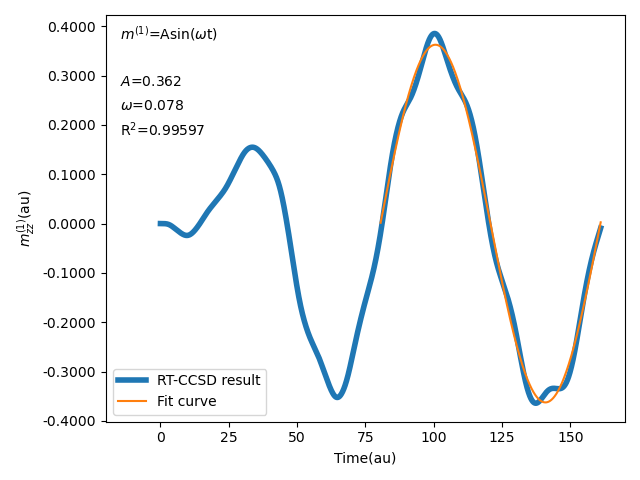
\includegraphics[width=\textwidth]{ch4/Figs/5-4.png}
     \end{subfigure}
     \caption{RT-CCSD/cc-pVDZ (dp) results of \ch{H_{2}} dimer obtained from four simulations with field strengths of 0.002 au, -0.002 au, 0.004 au, and -0.004 au. The left column displays the LRCW results, including the $z$ component of the induced magnetic dipole moment and the corresponding first-order dipole moments with their fitted curve. The right column presents the QRCW results.}
     \label{fig:g-fit}
\end{figure}
With our RT-CC implementation, we calculate the $G'$ tensor of the \ch{H_{2}} dimer using RT-CCSD and RT-CC3, both in single- and double-precision arithmetics. We employ both the LRCW and the QRCW for comparison purposes. As illustrated in Fig.~\ref{fig:g-fit}, we utilize the induced magnetic dipole moments from applied fields of varying strengths to compute the first-order magnetic dipole moments through the finite difference method, similar to the procedure for calculating polarizabilities. In this case, $G'_{zz}$ can be obtained from the magnetic dipole moment induced by the field applied in the $z$ direction, with its value represented by the amplitude of the fitted curve.

As per Table~\ref{tab:g-ccsd}, no distinction is observed between single- and double-precision results in the RT-CCSD calculations. The $G'$ tensor elements exhibit identical values for both the LRCW and the QRCW cases, with the distinction lying solely in the R$^{2}$ values. Notably, the QRCW significantly enhances curve fitting quality, aligning with the conclusion drawn in section~\ref{results-cc3-22}. Upon examining the example results in Fig.~\ref{fig:g-fit}, it is evident that the induced magnetic dipole moment curves are less smooth compared to the induced electric dipole moment curves discussed in the previous section. Particularly in the LRCW instance, a curvilinear trajectory of the dipole is observed. Although this irregular shape remains approximately periodic, it adversely affects curve fitting. A minor distortion is observed in the QRCW example, which has a lesser impact on curve fitting. Table~\ref{tab:g-cc3} presents the RT-CC3 results. Analogous to RT-CCSD, the disparities between single- and double-precision results are inconsequential. The QRCW enhances overall R$^{2}$ values and provides more dependable outcomes. Hence, the RT-CC3 method proves to be a viable approach for computing the $G'$ tensor and subsequently optical rotation.
% Table6-G' tensor
\begin{table}
  \centering
    \caption{RT-CCSD/cc-pVDZ $G'$ tensor elements (in atomic units) of H$_{2}$ dimer at 582 nm obtained using single- and double-precision computations, with linear ramped continuous wave (LRCW) and quadratic ramped continuous wave (QRCW) fields. The R$^{2}$ values, indicating the quality of curve fitting, are displayed in the last three columns.}
  \begin{tabular}{c|c|c|ccc}
                                          &  $G'$ & \textrm{RT-CCSD(dp)} & R$^{2}_{x}$(dp) & R$^{2}_{y}$(dp)& R$^{2}_{z}$(dp)\\
                                          \hline
                \textrm{LRCW} & ($G'_{xx}$, $G'_{yx}$, $G'_{zx}$) & (-0.387, -0.097, 0.000) &   0.93726 & 0.93911 & 0 \\
                                          & ($G'_{xy}$, $G'_{yy}$, $G'_{zy}$) & ( 0.058,  0.013, 0.000) &   0.88177 & 0.86203 & 0 \\
                                          & ($G'_{xz}$, $G'_{yz}$, $G'_{zz}$) & ( 0.000,  0.000, 0.362) &   0 & 0 & 0.93669 \\   
                \hline
                                           &  $G'$ & \textrm{RT-CCSD(sp)} & R$^{2}_{x}$(sp) & R$^{2}_{y}$(sp)& R$^{2}_{z}$(sp)\\
                                          \hline
                \textrm{LRCW} & ($G'_{xx}$, $G'_{yx}$, $G'_{zx}$) & (-0.387, -0.097, 0.000) &   0.93727 & 0.93911 & 0 \\
                                          & ($G'_{xy}$, $G'_{yy}$, $G'_{zy}$) & ( 0.058,  0.013, 0.000) &   0.88179 & 0.86205 & 0 \\
                                          & ($G'_{xz}$, $G'_{yz}$, $G'_{zz}$) & ( 0.000,  0.000, 0.362) &   0 & 0 & 0.93669 \\  
                 \hline
                                            &  $G'$ & \textrm{RT-CCSD(dp)} & R$^{2}_{x}$(dp) & R$^{2}_{y}$(dp)& R$^{2}_{z}$(dp)\\
                                          \hline
                \textrm{QRCW} & ($G'_{xx}$, $G'_{yx}$, $G'_{zx}$) & (-0.387, -0.097, 0.000) &   0.99956 & 0.99956 & 0 \\
                                          & ($G'_{xy}$, $G'_{yy}$, $G'_{zy}$) & ( 0.058,  0.013, 0.000) &   0.99915 & 0.99896 & 0 \\
                                          & ($G'_{xz}$, $G'_{yz}$, $G'_{zz}$) & ( 0.000,  0.000, 0.362) &   0 & 0 & 0.99597 \\  
                 \hline
                                            &  $G'$ & \textrm{RT-CCSD(sp)} & R$^{2}_{x}$(sp) & R$^{2}_{y}$(sp)& R$^{2}_{z}$(sp)\\
                                          \hline
                \textrm{QRCW} & ($G'_{xx}$, $G'_{yx}$, $G'_{zx}$) & (-0.387, -0.097, 0.000) &   0.99956 & 0.99956 & 0 \\
                                          & ($G'_{xy}$, $G'_{yy}$, $G'_{zy}$) & ( 0.058,  0.013, 0.000) &   0.99915 & 0.99896 & 0 \\
                                          & ($G'_{xz}$, $G'_{yz}$, $G'_{zz}$) & ( 0.000,  0.000, 0.362) &   0 & 0  & 0 .99597\\  
                
   \end{tabular}
  \label{tab:g-ccsd}
\end{table}
% Table7-G' tensor
\begin{table}
  \centering
    \caption{RT-CC3/cc-pVDZ $G'$ tensor elements (in atomic units) of H$_{2}$ dimer at 582 nm obtained using single- and double-precision computations, with linear ramped continuous wave (LRCW) and quadratic ramped continuous wave (QRCW) fields. The R$^{2}$ values, indicating the quality of curve fitting, are displayed in the last three columns.}
  \begin{tabular}{c|c|c|ccc}
                                          &  $G'$ & \textrm{RT-CC3(dp)} & R$^{2}_{x}$(dp) & R$^{2}_{y}$(dp)& R$^{2}_{z}$(dp)\\
                                          \hline
                \textrm{LRCW} & ($G'_{xx}$, $G'_{yx}$, $G'_{zx}$) & (-0.388, -0.097, 0.000) &   0.93805 & 0.93987 & 0 \\
                                          & ($G'_{xy}$, $G'_{yy}$, $G'_{zy}$) & ( 0.058,  0.013, 0.000) &   0.87896 & 0.85971 & 0\\
                                          & ($G'_{xz}$, $G'_{yz}$, $G'_{zz}$) & ( 0.000,  0.000, 0.363) &   0 & 0 & 0.93589 \\   
                \hline
                                           &  $G'$ & \textrm{RT-CC3(sp)} & R$^{2}_{x}$(sp) & R$^{2}_{y}$(sp)& R$^{2}_{z}$(sp)\\
                                          \hline
                \textrm{LRCW} & ($G'_{xx}$, $G'_{yx}$, $G'_{zx}$) & (-0.388, -0.097, 0.000) &   0.93805 & 0.93987 & 0 \\
                                          & ($G'_{xy}$, $G'_{yy}$, $G'_{zy}$) & ( 0.058,  0.013, 0.000) &   0.87896 & 0.85971 & 0 \\
                                          & ($G'_{xz}$, $G'_{yz}$, $G'_{zz}$) & ( 0.000,  0.000, 0.363) &   0 & 0 & 0.93588 \\  
                 \hline
                                            &  $G'$ & \textrm{RT-CC3(dp)} & R$^{2}_{x}$(dp) & R$^{2}_{y}$(dp)& R$^{2}_{z}$(dp)\\
                                          \hline
                \textrm{QRCW} & ($G'_{xx}$, $G'_{yx}$, $G'_{zx}$) & (-0.387, -0.097, 0.000) &   0.99955 & 0.99955 & 0 \\
                                          & ($G'_{xy}$, $G'_{yy}$, $G'_{zy}$) & ( 0.058,  0.013, 0.000) &   0.99911 & 0.99891 & 0 \\
                                          & ($G'_{xz}$, $G'_{yz}$, $G'_{zz}$) & ( 0.000,  0.000, 0.362) &   0 & 0 & 0.99602 \\  
                 \hline
                                            &  $G'$ & \textrm{RT-CC3(sp)} & R$^{2}_{x}$(sp) & R$^{2}_{y}$(sp)& R$^{2}_{z}$(sp)\\
                                          \hline
                \textrm{QRCW} & ($G'_{xx}$, $G'_{yx}$, $G'_{zx}$) & (-0.387, -0.097, 0.000) &   0.99955 & 0.99955 & 0 \\
                                          & ($G'_{xy}$, $G'_{yy}$, $G'_{zy}$) & ( 0.058,  0.013, 0.000) &  0.99911 & 0.99891 & 0 \\
                                          & ($G'_{xz}$, $G'_{yz}$, $G'_{zz}$) & ( 0.000,  0.000, 0.362) &   0 & 0 & 0.99602 \\  
                
   \end{tabular}
  \label{tab:g-cc3}
\end{table}

\subsection{Electron dynamics}\label{results-cc3-3}

In this section, we delve into the electron dynamics encompassing Rabi oscillations and the population of excited states within the RT-CC framework. We employ \ch{H_{2}}, \ch{LiH}, and \ch{C_{2}H_{4}} as our test cases. Our examination encompasses the effects of both the frequency and intensity of the external field. Furthermore, we investigate the stability and viability of the RT method, particularly in scenarios where the ground state is substantially depopulated. To validate our real-time implementation, we exclusively utilize the RT-CCSD method in double-precision. Employing a higher level of theory would be superfluous for the current objectives. Nevertheless, it's worth noting that the formalism employed for the RT-CCSD (dp) simulations can be seamlessly extended to RT-CC3 or single-precision calculations if necessitated.

\subsubsection{Rabi oscillation} \label{results-cc3-31}
%% H2-rabi
\subsubsubsection{\ch{H_{2}}} \label{results-cc3-311}
% Fig6: H2-abs
\begin{figure}
   \centering
   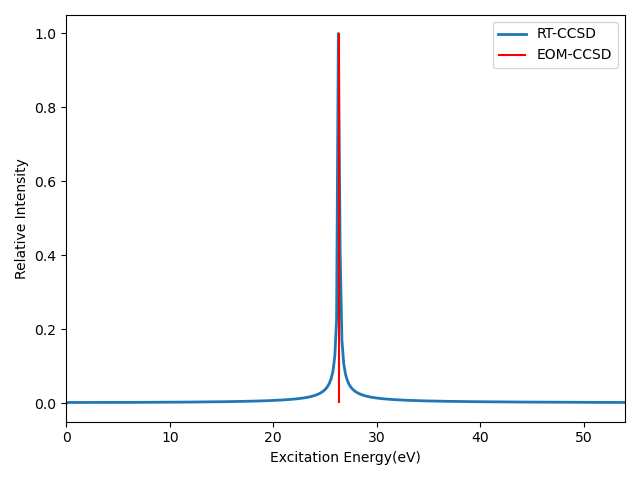
\includegraphics[angle=0, scale=0.45]{ch4/Figs/6-1.png}
   \label{fig:sp-monomer}
   \caption{RT-CCSD/STO-3G linear absorption spectrum of \ch{H_{2}} and corresponding EOM-CCSD/STO-3G transitions included as stick-spectra for comparison.}
     \label{fig:h2-abs}
\end{figure}
As a simple system comprising only two electrons, $H_{2}$ serves as an ideal molecule for testing the simulation of Rabi oscillations. We opt for a minimal basis set to eliminate complexities arising from multi-excited states. To initiate the excitation of one electron from the ground state to the excited state, we apply an oscillatory field to the system at a frequency of 0.976 au (equivalent to 26.56 eV). This frequency is determined through an EOM-CCSD/STO-3G calculation and is linked to the excitation energy of the $\sigma$-$\sigma^{*}$ transition, which is also visible in the spectrum depicted in Fig.~\ref{fig:h2-abs}. In this case, we apply the field for 500 au while varying the field strengths to observe the Rabi oscillation between the ground state S$_{0}$ and the singly-excited state S$_{1}$.

To characterize the patterns shown in Fig.~\ref{fig:h2-rabi}, we begin by examining the curves of the autocorrelation functions. It is evident that $|A(t_{0}, t)|^{2}$ oscillates between 0 and 1 for both cases. Furthermore, the Rabi frequency when the field strength is 0.0890 au (top right) is twice that of the case when the field strength is 0.0445 au (top left), which is consistent with the behavior of an ideal Rabi oscillation, where the Rabi frequency is proportional to the field strength of the driving field. Additionally, the relationship between the oscillation of the ground state population and the oscillation of the induced dipole is characteristic of Rabi oscillations. When S$_{0}$ and S$_{1}$ are equally populated, the amplitude of the dipole oscillation reaches its maximum. Conversely, when either S$_{0}$ or S$_{1}$ is fully populated, the amplitude of the dipole oscillation reaches its minimum. By observing the left and right columns of Fig.~\ref{fig:h2-rabi} respectively, it becomes apparent that the maximum amplitude in the dipole trajectory occurs when $|A(t_{0}, t)|^{2}=0.5$, and the minimum amplitude of the dipole coincides with the minima of $|A(t_{0}, t)|^{2}$ at zero or reaches the maxima at one. As demonstrated in the results, our RT-CCSD formalism successfully simulates the Rabi oscillation of \ch{H_{2}}.
% Fig7: H2-Rabi
\begin{figure}
     \centering
     \begin{subfigure}{0.47\textwidth}
         \centering
         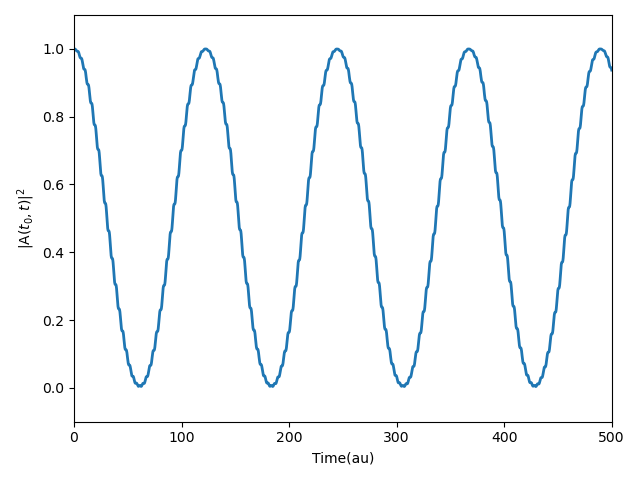
\includegraphics[width=\textwidth]{ch4/Figs/7-1.png}
     \end{subfigure}
     \hfill
     \begin{subfigure}{0.47\textwidth}
         \centering
         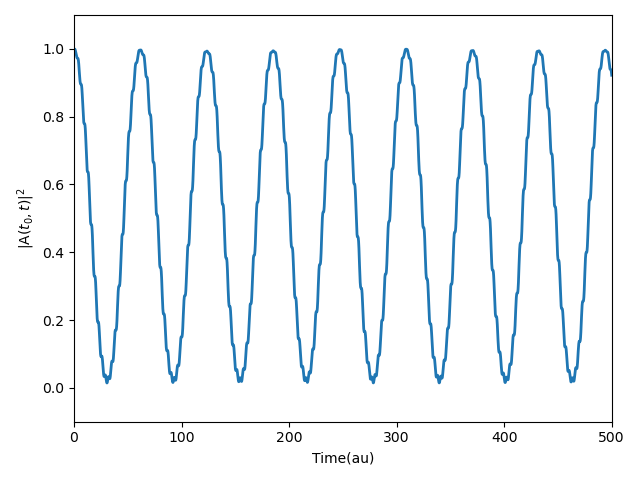
\includegraphics[width=\textwidth]{ch4/Figs/7-3.png}
      \end{subfigure}
       \vfill
     \begin{subfigure}{0.47\textwidth}
         \centering
         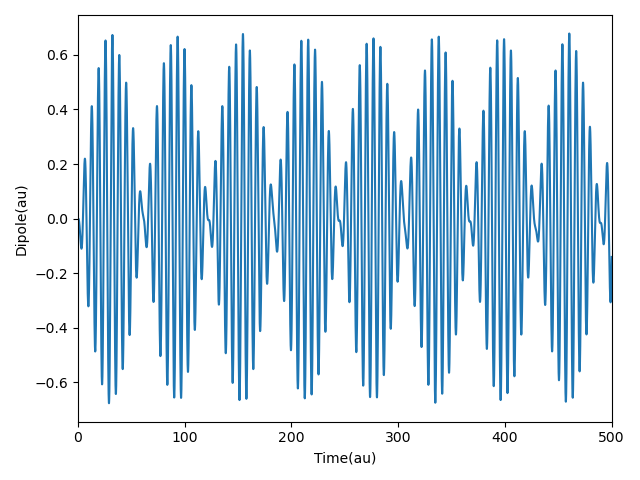
\includegraphics[width=\textwidth]{ch4/Figs/7-2.png}
     \end{subfigure}
     \hfill
     \begin{subfigure}{0.47\textwidth}
         \centering
         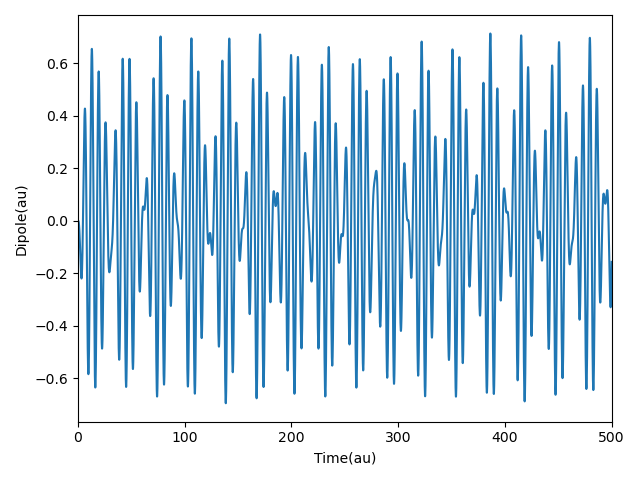
\includegraphics[width=\textwidth]{ch4/Figs/7-4.png}
     \end{subfigure}
     \caption{Rabi oscillation simulations of \ch{H_{2}} with external fields having intensities of 0.0445 au (left column) and 0.0890 au (right column). The first row displays results of $|A(t_{0}, t)|^{2}$ to indicate the population of the ground state at time $t$. The second row shows the corresponding induced dipole.}
     \label{fig:h2-rabi}
\end{figure}
%% C2H4-rabi
\subsubsubsection{\ch{C_{2}H_{4}}}\label{results-cc3-312}
With the existing formalism, \ch{C_{2}H_{4}} is also an interesting test case for Rabi oscillation. As a multi-electron molecule, it does not have the basic energy levels like \ch{H_{2}}. However, the $\pi$ and $\pi^{*}$ orbitals of the double bond can be approximately viewed as a two-level system. The calculation is conducted with the core orbitals frozen for efficiency. The number of active occupied orbitals and virtual orbitals is 6 each, using the STO-3G basis set. The frequency of the field is chosen to be 0.489 au (13.31 eV), which corresponds to the lowest excitation energy, corresponding to the $\pi$-$\pi^{*}$ transition as shown in the absorption spectrum in Fig.~\ref{fig:c2h4-abs}.
% Fig11: C2H4-abs
\begin{figure}
   \centering
   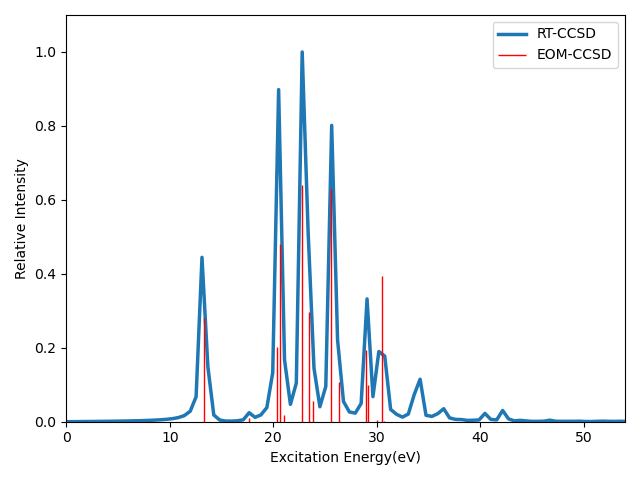
\includegraphics[angle=0, scale=0.43]{ch4/Figs/8-1.png}
   \caption{RT-CCSD/STO-3G linear absorption spectrum of \ch{C_{2}H_{4}} and corresponding EOM-CCSD/STO-3G transitions included as stick-spectra for comparison.}
     \label{fig:c2h4-abs}
\end{figure}

From the EOM-CCSD/STO-3G calculation, the leading contribution of this EOM state is the excitation from the highest occupied molecular orbital (HOMO) to the lowest unoccupied molecular orbital (LUMO), which corresponds to the specific $\hat{T}_{1}$ amplitude, $t_{5}^{0}$. Note that the orbital numbering starts from zero; thus, $t_{5}^{0}$ is associated with the sixth occupied orbital, the HOMO, and the first unoccupied orbital, the LUMO. If the state of the molecule at time $t$ can be expanded as a linear combination of all stationary point states, $t_{5}^{0}$ is the leading term of the coefficient of the lowest excited state. $|t_{5}^{0}|^{2}$ can thus be viewed as the population of this specific state. 

An additional autocorrelation function can be formulated using the ground state and a state vector with $t_{5}^{0}$ being the only nonzero amplitude at time $t$. Fig.~\ref{fig:c2h4-rabi} shows the population of the ground state on the left and the probability of the $\pi$-$\pi^{*}$ transition on the right. Unlike the success in simulating the Rabi oscillation of \ch{H_2}, the propagation is numerically unstable. From the figure on the left, the square of the autocorrelation function initially decreases from 1, reaches its minimum around 0.13, and then increases drastically, leading to a failure of the propagation.

In previous works on RT-CC methods, it has been demonstrated that the depletion of the ground state can cause a crash of the calculation. CC takes the ground state as the leading and reference state, while the ground state is no longer the most populated state due to the external field.\cite{Kristiansen2020} Although the value of the autocorrelation function does not diverge precisely at its minimum around 290 au, the population of the lowest excited state shown on the right confirms that $|t_{5}^{0}|^{2}$ diverges more rapidly as it moves beyond 0.5 and approaches one around 290 au. 

It is not clear why the simulation fails for the approximate Rabi oscillation of \ch{C_{2}H_{4}}, while it works for the Rabi oscillation of \ch{H_{2}}. Orbital-optimized methods may be good candidates for this situation, as they have been shown to work well for applying intense external fields when the population of the ground state approaches zero.\cite{Kristiansen2020} Such methods may also help identify the discrepancy between the approximate two-level system in the double bond and the exact two-level system. Further exploration is needed. 
% Fig10: C2H4-Rabi
\begin{figure}
     \centering
     \begin{subfigure}{0.45\textwidth}
         \centering
         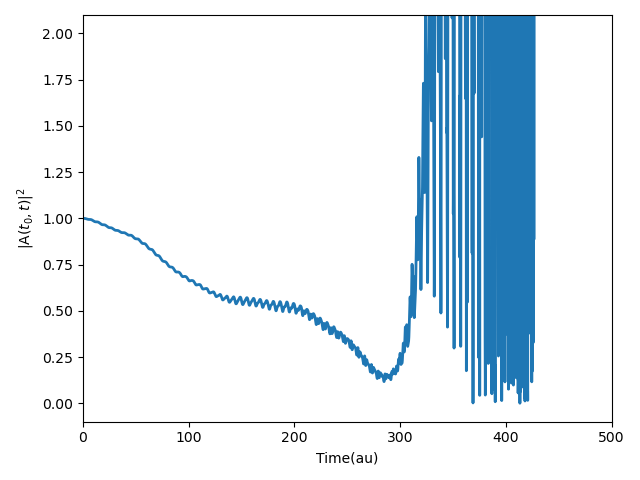
\includegraphics[width=\textwidth]{ch4/Figs/9-1.png}
     \end{subfigure}
     \hfill
     \begin{subfigure}{0.45\textwidth}
         \centering
         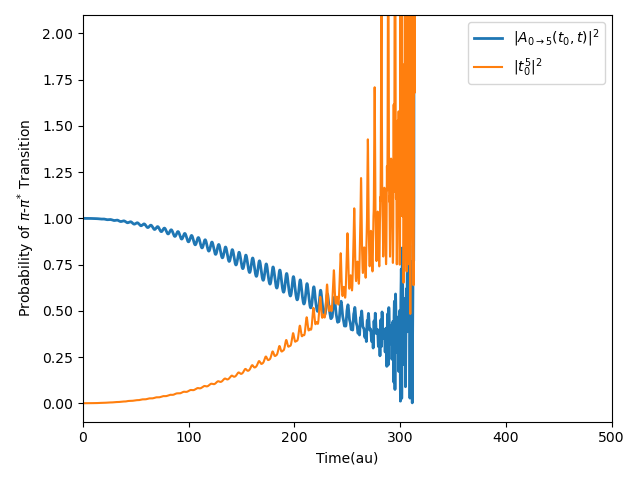
\includegraphics[width=\textwidth]{ch4/Figs/9-2.png}
      \end{subfigure}
     \caption{Rabi oscillation simulation of \ch{C_{2}H_{4}}. The intensity and frequency of the external field are chosen to be 0.01 au and 0.489 au, respectively. The left figure displays $|A(t_{0}, t)|^{2}$, indicating the population of the ground state at time $t$. The right one shows the probability of the targeted $\pi$-$\pi^{*}$ transition, represented by the square of the autocorrelation function and the square of $\hat{T}_{1}$ amplitude associated with the transition. The simulation lasts for 500 au, with the `cut off' of the curve indicating the time when the values diverge.}
     \label{fig:c2h4-rabi}
\end{figure}

\subsubsection{Population of the excited states}\label{results-cc3-32}
%%H2-ge
\subsubsubsection{\ch{H_{2}}}\label{results-cc3-321}
% Fig8: H2-Rabi-g-e
\begin{figure}
     \centering
     \begin{subfigure}{0.47\textwidth}
         \centering
         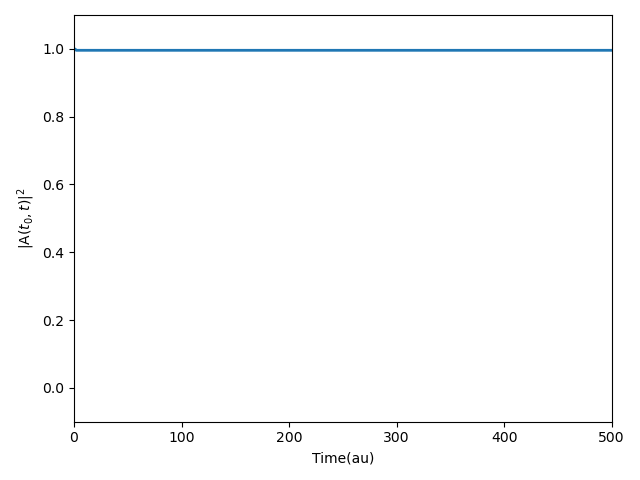
\includegraphics[width=\textwidth]{ch4/Figs/10-1.png}
     \end{subfigure}
     \hfill
     \begin{subfigure}{0.47\textwidth}
         \centering
         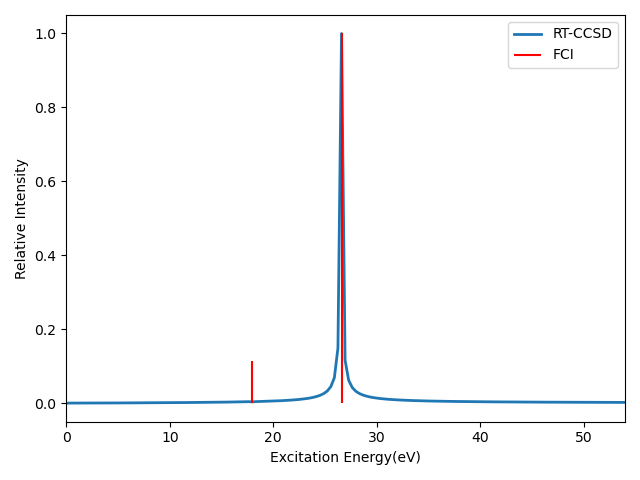
\includegraphics[width=\textwidth]{ch4/Figs/10-2.png}
      \end{subfigure}
       \vfill
     \begin{subfigure}{0.47\textwidth}
         \centering
         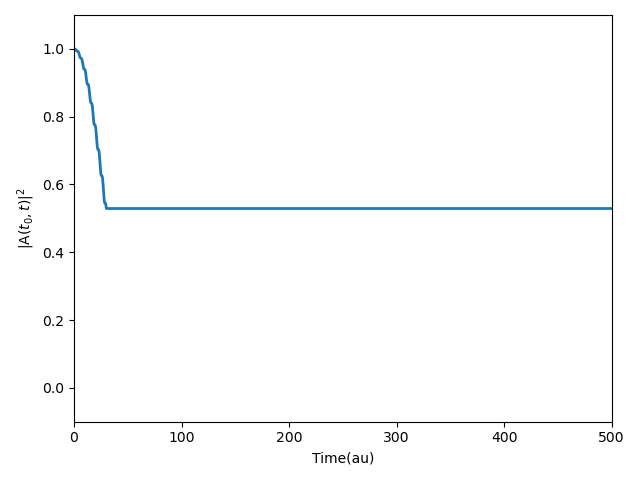
\includegraphics[width=\textwidth]{ch4/Figs/10-3.png}
     \end{subfigure}
     \hfill
     \begin{subfigure}{0.47\textwidth}
         \centering
         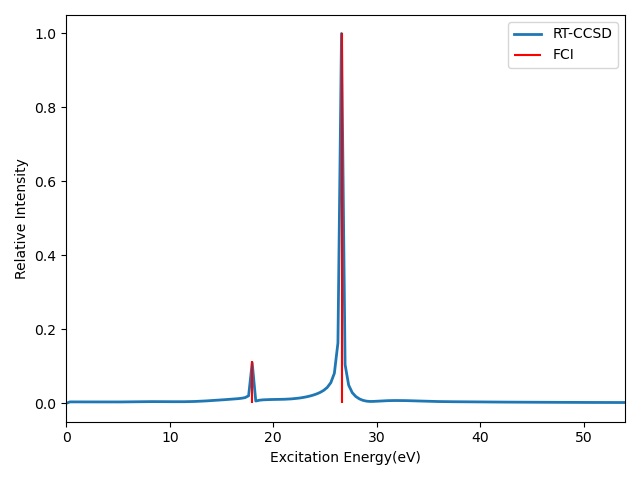
\includegraphics[width=\textwidth]{ch4/Figs/10-4.png}
     \end{subfigure}
      \vfill
     \begin{subfigure}{0.47\textwidth}
         \centering
         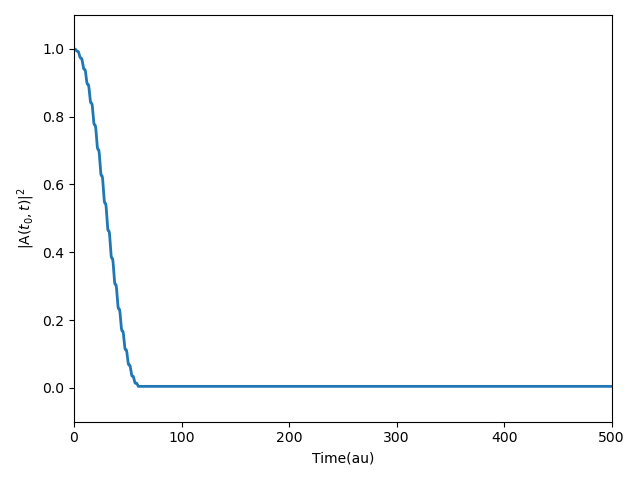
\includegraphics[width=\textwidth]{ch4/Figs/10-5.png}
     \end{subfigure}
     \hfill
     \begin{subfigure}{0.47\textwidth}
         \centering
         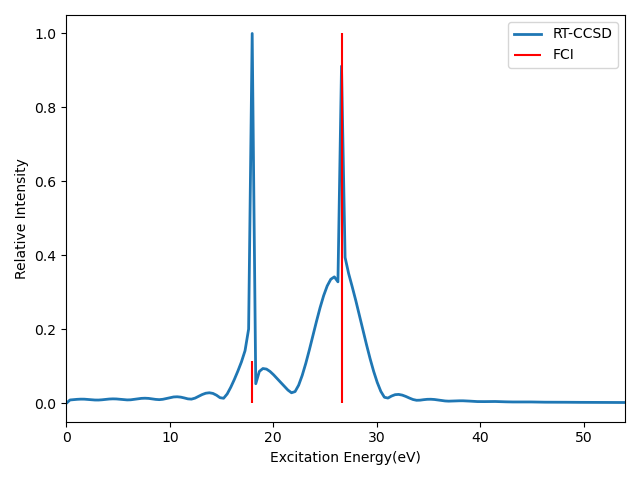
\includegraphics[width=\textwidth]{ch4/Figs/10-6.png}
     \end{subfigure}
     \caption{RT-CCSD/STO-3G results of \ch{H_{2}} with the external field applied for 2 au, 30 au, and 60 au. The left column displays the results of $|A(t_{0}, t)|^{2}$, indicating the population of the ground state at time $t$. The right column shows the corresponding absorption spectra. FCI/STO-3G transitions are included as stick spectra for comparison.}
     \label{fig:h2-ge}
\end{figure}
Besides the Rabi oscillation itself, details about the population of each state can provide additional information about the electron dynamics. To target different state populations in the RT propagation, the duration of the applied field can be varied according to the Rabi frequency obtained from the Rabi oscillation simulation. As shown in Fig.~\ref{fig:h2-ge}, the propagations are run for a total of 500 au. The field lasts for 2 au, 30 au, or 60 au, with the resulting $|A(t_{0}, t)|^{2}$ and absorption spectrum shown in the first, second, and third rows of Fig.~\ref{fig:h2-ge}, respectively.

When the field is turned off after only 2 au, $|A(t_{0}, t)|^{2}$ decreases slightly and remains close to 1 for the rest of the propagation. The resulting absorption spectrum reflects the singly-excited state correctly. When the duration of the field is increased to 30 au, $|A(t_{0}, t)|^{2}$ can be reduced to around 0.5, indicating a 50\% chance of finding the molecule in its ground state. A second peak appears in the lower frequency region of the spectrum. When the field is on for 60 au, the ground state is depleted, as shown by the decline of $|A(t_{0}, t)|^{2}$ from one to zero. As the duration of the field increases, the secondary peak becomes more prominent. The quality of the absorption spectrum is also diminished due to the deviation from the ground state.

In addition, the density matrix can be utilized to check the population of different states, as the diagonal elements represent the occupation numbers of the molecular orbitals. When the field is switched off after 2 au, the occupation number of the occupied orbital (OO) becomes 1.971, while the occupation number of the virtual orbital (OV) becomes 0.029, which is not far from the ground state. For the calculation where the field lasts for 30 au, NO$=1.496$ and NV$=0.504$. For the 60 au case, NO$=0.999$ and NV$=1.001$. The sum of NO and NV is the total number of electrons. These values are consistent with the corresponding autocorrelation functions. However, this does not explain the additional peak in the absorption spectra.

To identify the excited states, FCI results from Ref.~\citenum{Provorse2015} are included as stick spectra. In Ref.~\citenum{Provorse2015}, Provorse et al. discussed the population of the doubly-excited state S$_{2}$ from both TDCI and RT-TDDFT simulations of the Rabi oscillation, where RT-TDDFT has an artificial peak shift due to the limitation of the exchange functional. For our RT-CCSD calculation, the left and right peaks match the excitation energy from S$_{1}$ to S$_{2}$ and the excitation energy from S$_{0}$ to S$_{1}$, respectively. For an EOM-CCSD calculation with the RHF reference, only one transition from S$_{0}$ to S$_{1}$ can be obtained. The spectrum shows that the population of S$_{2}$ is not zero and increases with the decrease in ground state population induced by the applied field. The excitation energy can be obtained from the absorption spectrum, although the implementation is built upon an RHF formalism.
%% LiH-ge
\subsubsubsection{\ch{LiH}}\label{results-cc3-322}
To further explore the transitions to excited states caused by the external field, an oscillatory field is applied to \ch{LiH} for one optical cycle. The frequency is chosen to be the excitation energy associated with the $\sigma$-$\sigma^{*}$ transition, which is 0.652 au as obtained from the EOM-CCSD/STO-3G calculation. The duration of the field is therefore 9.64 au, while the total length of the propagation is 500 au. A reference absorption spectrum with a thin Gaussian pulse as the applied field is shown in Fig.~\ref{fig:lih-abs}, where the peaks match the EOM-CCSD results for the ground state to excited state transitions.

As shown in the left column of Fig.~\ref{fig:lih-ge}, the population of the ground state decreases with the increase in the field strength, resulting in a larger probability of ground state to excited state and excited state to excited state transitions. In the resulting absorption spectra on the right, in addition to the ground to excited state transitions, the excited to excited state transitions, labeled as thinner sticks for the reference value, are found and become more populated when the field strength is increased to 0.15 au. If the intensity is further increased to 0.45 au, some of the transitions become more obvious, but the stability of the propagation and the line shape of the spectrum are no longer ideal.

Overall, the RT-CCSD calculation can recover most of the excited state to excited state transitions, although they are still weaker than the ground state to excited state transitions. A reasonable field strength needs to be selected to ensure that the electrons can be excited while retaining the stability of the calculation.
% Fig9: LiH-abs
\begin{figure}
   \centering
   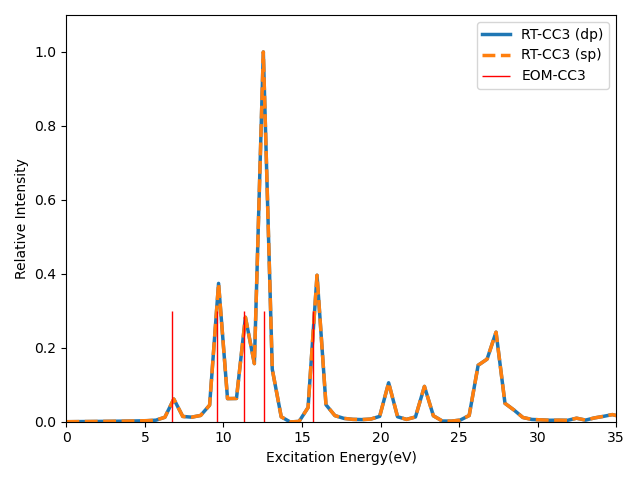
\includegraphics[angle=0, scale=0.43]{ch4/Figs/1-1.png}
   \caption{RT-CCSD/STO-3G linear absorption spectrum of \ch{LiH} and corresponding EOM-CCSD/STO-3G transitions included as stick-spectra for comparison.}
     \label{fig:lih-abs}
\end{figure}
% Fig10: LiH-g-e
\begin{figure}
     \centering
     \begin{subfigure}{0.47\textwidth}
         \centering
         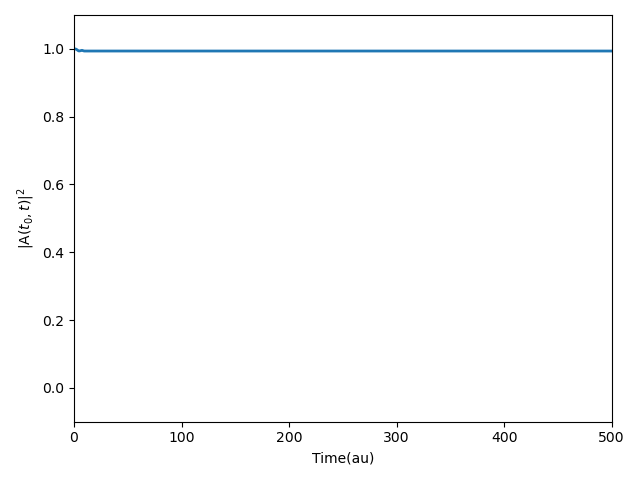
\includegraphics[width=\textwidth]{ch4/Figs/12-1.png}
     \end{subfigure}
     \hfill
     \begin{subfigure}{0.47\textwidth}
         \centering
         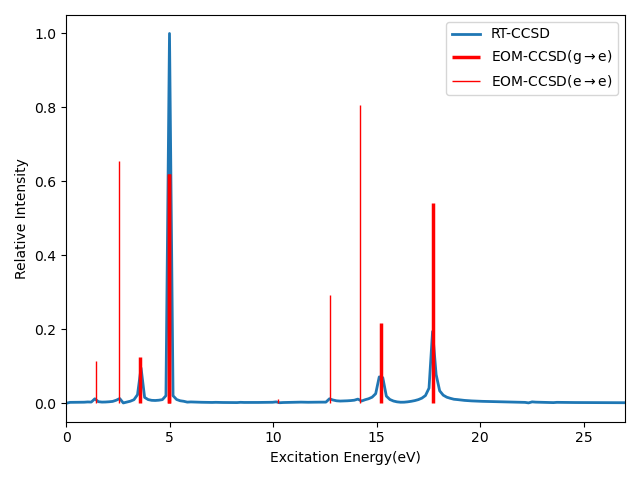
\includegraphics[width=\textwidth]{ch4/Figs/12-2.png}
      \end{subfigure}
       \vfill
     \begin{subfigure}{0.47\textwidth}
         \centering
         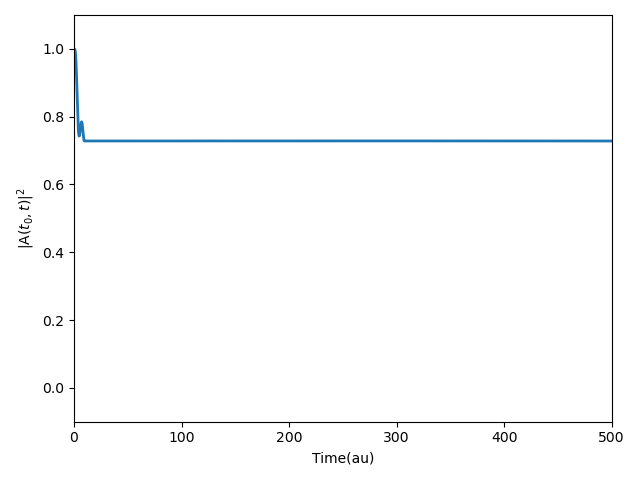
\includegraphics[width=\textwidth]{ch4/Figs/12-3.png}
     \end{subfigure}
     \hfill
     \begin{subfigure}{0.47\textwidth}
         \centering
         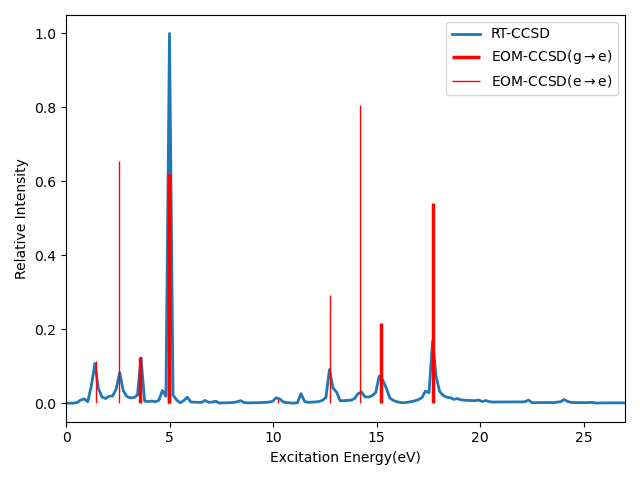
\includegraphics[width=\textwidth]{ch4/Figs/12-4.png}
     \end{subfigure}
      \vfill
     \begin{subfigure}{0.47\textwidth}
         \centering
         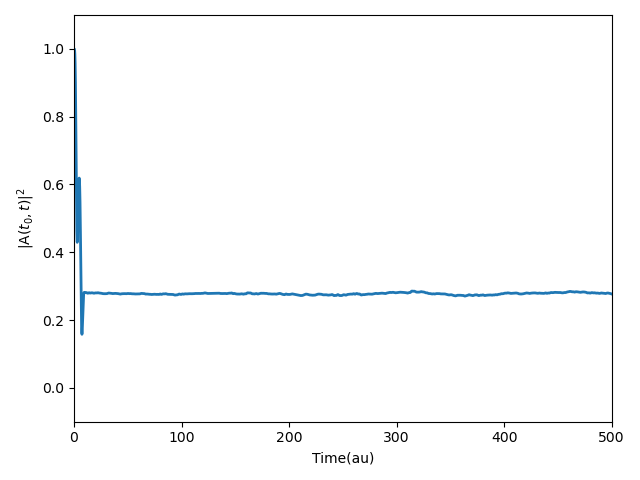
\includegraphics[width=\textwidth]{ch4/Figs/12-5.png}
     \end{subfigure}
     \hfill
     \begin{subfigure}{0.47\textwidth}
         \centering
         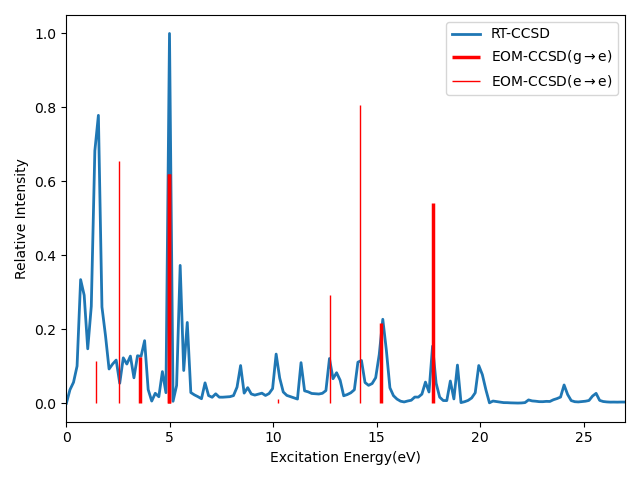
\includegraphics[width=\textwidth]{ch4/Figs/12-6.png}
     \end{subfigure}
     \caption{RT-CCSD/STO-3G results of \ch{LiH} with external fields of varying intensities (0.01 au, 0.15 au, and 0.45 au) applied for a duration of 500 au. The left column displays the evolution of the ground state population $|A(t_{0}, t)|^{2}$ over time $t$, while the right column showcases the corresponding absorption spectra. Stick-spectra of EOM-CCSD/STO-3G transitions are included for comparison.}
     \label{fig:lih-ge}
\end{figure}